\documentclass[11pt,reqno]{amsart}

\usepackage[utf8]{inputenc}
\usepackage[T1]{fontenc}
\usepackage{lmodern}
\usepackage{amsmath,amssymb,amsfonts,amsthm,mathtools}
\usepackage{booktabs,array,multirow}
\usepackage{graphicx}
\usepackage{enumitem}
\usepackage[margin=1.0in]{geometry}
\usepackage{microtype}
\usepackage{xcolor}
\definecolor{linkblue}{rgb}{0.0,0.2,0.6}
\usepackage[colorlinks=true,linkcolor=linkblue,citecolor=linkblue,urlcolor=linkblue]{hyperref}

\newtheorem{theorem}{Theorem}[section]
\newtheorem{proposition}[theorem]{Proposition}
\newtheorem{lemma}[theorem]{Lemma}
\newtheorem{corollary}[theorem]{Corollary}
\theoremstyle{definition}
\newtheorem{definition}[theorem]{Definition}
\theoremstyle{remark}
\newtheorem{remark}[theorem]{Remark}

\numberwithin{equation}{section}
\allowdisplaybreaks

\newcommand{\R}{\mathbb{R}}
\newcommand{\C}{\mathbb{C}}
\newcommand{\N}{\mathbb{N}}
\newcommand{\Z}{\mathbb{Z}}
\newcommand{\dd}{\mathrm{d}}
\newcommand{\ee}{\mathrm{e}}
\newcommand{\ii}{\mathrm{i}}
\newcommand{\Rea}{\mathrm{Re}}
\newcommand{\Ima}{\mathrm{Im}}
\newcommand{\rad}{\mathrm{rad}}
\newcommand{\sinch}{\mathrm{sinc}_{\mathrm{hyp}}}
\newcommand{\fac}{\mathclose{\mathchar"0021}}

\title[Bilinear Rank-2 Wronskian Factorization and Pure-Square Completion]{Bilinear Rank-2 Factorization of Integrated Wronskian Kernels, Pure-Square Completion, and the $1+2d > 1$ Montgomery--Vaughan Exponent Jump in the Critical Strip}

\author{Thijs Missiaen}
\address{Independent Researcher, Belgium}
\email{thijs.missiaen@gmail.com}
\thanks{ORCID: \href{https://orcid.org/0009-0007-3678-0810}{0009-0007-3678-0810}}

\subjclass[2020]{Primary 11M06, 11N36; Secondary 30D15, 42A05}
\keywords{Riemann $\Xi$-function, transverse Wronskian, bilinear rank-2 factorization, pure-square completion, generalized von Mangoldt function, Montgomery--Vaughan Hilbert inequality, Preissmann constant, Gallagher--Sobolev inequality}
\dedicatory{\upshape October 25, 2026}
\date{October 25, 2026}

\begin{document}
\sloppy

\begin{abstract}
We study the off-diagonal cross-terms of the parity-reduced Wronskian $\widetilde{W}_{\mathcal{M}}(d,t)$ and its integral $\widetilde{\mathcal{E}}_{\mathcal{M}}(d,t)$ for Riemann's $\Xi$-function on $d \in (0, \frac{1}{2}]$. First, every off-diagonal pair $1 \le m < n \le N(t) = \lfloor\sqrt{t/2\pi}\rfloor$ obeys $\mathcal{H}_{mn}^+(d,t)/\mathcal{D}_{1,1}(d,t) < (mn)^{-d} \le 2^{-d} < 1$, and the integrated cross-term kernel factors into the bilinear rank-2 form $w_{mn}^{\mathrm{int}}(d,t) \equiv 2d^{-2}(\cosh(d\omega_m(t))\cosh(d\omega_n(t)) - 1)$, reducing $\mathcal{O}(N(t)^2)$ double sums to $\mathcal{O}(N(t))$ sums with a phase transition $N(t)^{1-4d}$ at $d = \frac{1}{4}$. Second, adding the critical-line ground state cancels the $-1$ boundary term pair by pair, completing the $(m,n \ge 2)$ sector into the pure square $+d^{-2}\|\Psi_{\ge 2}(d,t)\|^2 \ge 0$ and eliminating the $1 + \sqrt{2}$ penalty. Finally, passing from $L^1$ to $L^2$ jumps the exponent from $\frac{1}{2} + d < 1$ to $1 + 2d > 1$ for all $d > 0$, which with Preissmann's Hilbert constant $c_{\mathrm{MV}} = \frac{4}{3}\sqrt{6}$ on windows $\Delta T_{\mathrm{MV}}(d,t) \asymp N(t)^{1-2d} = o(t^{1/2})$ gives $X_{\mathrm{MV},\infty}^{(r)}(d) = \mathcal{O}(1)$ and $\theta_{\mathrm{MV}}^{(r)}(d,t) = \mathcal{O}(1/\ln t) \to 0$.
\end{abstract}

\maketitle

\section{Introduction and Main Results}\label{sec:intro}

In the analytic theory of the Riemann zeta function $\zeta(s)$ ($s = \sigma + \ii t = \frac{1}{2} + d + \ii t$) and Riemann's completed function $\Xi(z) := \xi(\frac{1}{2} + \ii z) = R(d,t) + \ii\,I(d,t)$ ($z = t - \ii d$)~\cite{riemann1859,titchmarsh1986}, the monotonicity of $|\Xi(t - \ii d)|^2$ away from the critical line $d = 0$ is governed by the transverse Wronskian
\begin{equation}\label{eq:intro_wronskian}
W(d,t) := \frac{1}{2}\frac{\partial}{\partial d}\bigl|\Xi(t - \ii d)\bigr|^2 = R\,\partial_d R + I\,\partial_d I = R\,\partial_t I - I\,\partial_t R,
\end{equation}
whose strict positivity for $d > 0$ is equivalent to the Speiser--Hinkkanen--Lagarias monotonicity criterion $\Rea(\xi'(s)/\xi(s)) > 0$~\cite{speiser1934,hinkkanen1997,lagarias1999} and closely linked to the P\'olya--Jacobi kernel $\Phi(u)$~\cite{jacobi1829,polya1926}, Tur\'an--Jensen total positivity~\cite{csordas1986}, Wigner phase-space quasi-probabilities~\cite{wigner1932,hudson1974}, and de~Branges Hilbert spaces~\cite{conreyli2000}. In Papers~I--VII of this series~\cite{missiaen2026paper1,missiaen2026paper2,missiaen2026paper3,missiaen2026paper4,missiaen2026paper5,missiaen2026paper6,missiaen2026paper7}, we introduced the parity-reduced Wronskian $\widetilde{W}(d,t) := W(d,t)/d$, the universal mother-wavelet decomposition $\Phi(u) = \sum_{n=1}^{\infty} n^{-1/2}\varphi_1(u + \frac{1}{2}\ln n)$, and finite-divisor sieved multipliers $\mathcal{M}(z)$ preserving critical-line mirror symmetry.

When the mother-wavelet expansion of $\Xi_{\mathcal{M}}(z) := \Xi(z)\mathcal{M}(z)$ is evaluated via complex saddle points up to the Riemann--Siegel horizon $N(t) := \lfloor\sqrt{t/2\pi}\rfloor$~\cite{siegel1932,gabcke1979}, the parity-reduced transverse gradient decomposes into a strictly positive, oscillation-free diagonal ($m = n$) and $\binom{N(t)}{2}$ oscillatory off-diagonal cross-pairs ($1 \le m < n \le N(t)$). Controlling these $\binom{N(t)}{2}$ off-diagonal pairs across the critical strip $0 < d \le \frac{1}{2}$ as $t \to \infty$ confronts four fundamental analytical questions:
\begin{enumerate}[label=\textup{(\arabic*)},leftmargin=2.2em]
\item \textit{Quadratic pair complexity $\mathcal{O}(N(t)^2)$ and hyperbolic off-diagonal scaling.} At height $t = 10^8$ ($N(t) = 3989$), there are $\binom{3989}{2} = 7{,}954{,}066$ active cross-pairs $(m,n)$, each weighted by coupled hyperbolic frequencies $\omega_{mn}^+(t) = \frac{1}{2}\ln\frac{t}{2\pi mn}$ and $\omega_{mn}^- = \frac{1}{2}\ln\frac{n}{m}$. Can the integrated off-diagonal kernel be factored exactly into separable one-dimensional sums in $m$ and $n$?
\item \textit{The $(m,n \ge 2)$ mutual cross-term sign problem and the $1 + \sqrt{2}$ root penalty.} In worst-case triangle-inequality bounds, assigning a simultaneous minus sign to both the $(1,n)$ cross-sum $-S_{1,\mathrm{off}}/u$ and the $(m,n \ge 2)$ mutual cross-sum $-S_{2,\mathrm{off}}/u^2$ ($u = (\ln X)^r$) produces the quadratic equation $1 - 2Y - Y^2 = 0$, inflating the critical sieve threshold by $1 + \sqrt{2} \approx 2.41421356$. Can the $(m,n \ge 2)$ sector actually become negative?
\item \textit{The Euler--Maclaurin phase transition at $d = \frac{1}{4}$ ($\sigma = \frac{3}{4}$).} How do the integrated off-diagonal sums $S_{1,\mathrm{off}}^{\mathrm{int},(r)}(d,t)$ and $S_{2,\mathrm{off}}^{\mathrm{int},(r)}(d,t)$ scale relative to the ground-state diagonal $\mathcal{D}_{1,1}^{\mathrm{int}}(d,t) \sim \frac{1}{2d^2}N(t)^{2d}$ across the inner strip $d \in (0, \frac{1}{4})$ versus the outer strip $d \in (\frac{1}{4}, \frac{1}{2}]$?
\item \textit{Overcoming the $L^1$ divergence barrier $\frac{1}{2} + d < 1$ inside $0 < d < \frac{1}{2}$.} Because individual harmonic amplitudes scale as $|b_n|n^{-(1/2+d)}$, any phase-blind $L^1$ triangle inequality diverges as $N(t)^{1/2-d}$ for $0 < d < \frac{1}{2}$~\cite{selberg1942,levinson1974,conrey1989}. How does incorporating phase oscillation via the Montgomery--Vaughan--Preissmann Hilbert inequality~\cite{montgomeryvaughan1974,preissmann1984} and Gallagher's Sobolev inequality~\cite{gallagher1970} alter the critical exponent across $d > 0$?
\end{enumerate}

In the present paper (Paper~VIII), we resolve all four questions analytically and computationally up to $t = 10^8$. Our main results are summarized in the following theorem.

\begin{theorem}[Bilinear Rank-2 Factorization, Pure-Square Completion, and the $1+2d > 1$ Exponent Jump]\label{thm:main}
Let $s = \frac{1}{2} + d + \ii t$ and $z = t - \ii d$ with $d > 0$ and $t > 4\pi$, let $L := \ln(t/2\pi)$, $x_t := \sqrt{t/2\pi}$, $N(t) := \lfloor x_t\rfloor$, and $\omega_n(t) := \frac{1}{2}\ln\frac{t}{2\pi n^2} = \frac{1}{2}L - \ln n$ for $1 \le n \le N(t)$. Under the smooth order-$r$ M\"obius filter $P_r(x) = 1 - (1-x)^r$ ($r \in \N_{\ge 1}$) with sieved coefficients $b_n^{(r)}(X) = \sum_{k \mid n,\, k \le X} \mu(k)P_r(\frac{\ln(X/k)}{\ln X})$, the following four structural laws hold unconditionally:
\begin{enumerate}[label=\textup{(\roman*)},leftmargin=2.2em]
\item \textbf{Universal $(mn)^{-d} \le 2^{-d}$ Hyperbolic Diagonal Advantage and Order-$r$ Generalized von Mangoldt Scaling.} In the parity-reduced Riemann--Siegel mirror gradient, every off-diagonal pair $1 \le m < n \le N(t)$ satisfies the exact decomposition $\sinh(2d\omega_{mn}^+(t)) \equiv (mn)^{-d}\sinh(2d\omega_1(t)) - \sinh(d\ln(mn))(t/2\pi)^{-d}$ and the universal pointwise inequality
\begin{equation}\label{eq:intro_hyp_adv}
\frac{\mathcal{H}_{mn}^+(d,t)}{\mathcal{D}_{1,1}(d,t)} < \left(1 - \frac{\ln(mn)}{\ln(t/2\pi)}\right)(mn)^{-d} < (mn)^{-d} \le 2^{-d} < 1 \qquad (\forall\, d > 0).
\end{equation}
Moreover, $b_1^{(r)}(X) \equiv 1$ and $b_n^{(r)}(X) = \frac{\Lambda_r(n)}{(\ln X)^r}$ for all $2 \le n \le X$, where $\Lambda_r(n) := -\sum_{k \mid n} \mu(k)(\ln k)^r$ obeys the parity alternation law $|\Lambda_r(n)| \equiv (-1)^{\omega(n)-1}\Lambda_r(n) \ge 0$, vanishes identically whenever $\omega(n) > r$, satisfies the radical bound $|\Lambda_r(n)| \le (\ln\rad(n))^r \le (\ln n)^r$, and obeys the Stirling--Dirichlet convolution asymptotics $\sum_{n \le x} |\Lambda_r(n)| \sim \bigl(\sum_{m=1}^r \frac{1}{(r-1)\fac}\bigl[\begin{smallmatrix} r \\ m \end{smallmatrix}\bigr]\bigr)x(\ln x)^{r-1} = r\,x\,(\ln x)^{r-1}$.
\item \textbf{Exact Bilinear Rank-2 Factorization of Integrated Wronskian Kernels and Phase Transition at $d = \frac{1}{4}$.} Under the hyperbolic low-pass filter $\mathcal{F}_{\mathrm{int}}(x) := \frac{\tanh(x/2)}{x/2} \in (0, 1)$ of the integrated sieved energy clamp $\widetilde{\mathcal{E}}_{\mathcal{M}}(d,t) := \frac{1}{d^2}|\Xi_{\mathcal{M}}(t)|^2 + \frac{2}{d^2}\int_0^d u\,\widetilde{W}_{\mathcal{M}}(u,t)\,\dd u$, the integrated Gabcke--Olver remainder is damped relative to the leading diagonal by $\cosh^{-2}(\frac{1}{4}dL) < 1$, and the integrated off-diagonal weight factors identically into the bilinear rank-2 form
\begin{equation}\label{eq:intro_rank2}
w_{mn}^{\mathrm{int}}(d,t) \equiv \frac{2\bigl(\cosh(d\omega_m(t))\cosh(d\omega_n(t)) - 1\bigr)}{d^2} \qquad (1 \le m < n \le N(t)).
\end{equation}
Consequently, the $\mathcal{O}(N(t)^2)$ double sums $S_{1,\mathrm{off}}^{\mathrm{int},(r)}(d,t)$ and $S_{2,\mathrm{off}}^{\mathrm{int},(r)}(d,t)$ reduce identically to the $\mathcal{O}(N(t))$ one-dimensional sums $\Sigma_{\cosh}^{(r)}(d,t) := \sum_{n=2}^{N(t)} \frac{|\Lambda_r(n)|}{\sqrt{n}}\cosh(d\omega_n(t))$ and $\Sigma_0^{(r)}(t) := \sum_{n=2}^{N(t)} \frac{|\Lambda_r(n)|}{\sqrt{n}}$, and satisfy for $d \in (0, \frac{1}{2})$ as $N(t) \to \infty$:
\begin{equation}\label{eq:intro_phase_trans}
\begin{aligned}
\frac{S_{1,\mathrm{off}}^{\mathrm{int},(r)}(d,t)}{\mathcal{D}_{1,1}^{\mathrm{int}}(d,t)} &\sim \frac{8r}{1 - 4d^2}\,N(t)^{\frac{1}{2}-d}\bigl(\ln N(t)\bigr)^{r-1}, \\
\frac{S_{2,\mathrm{off}}^{\mathrm{int},(r)}(d,t)}{\bigl(\mathcal{D}_{1,1}^{\mathrm{int}}(d,t)\bigr)^2} &\sim \frac{256r^2 d^4(1 - 2d^2)}{(1 - 4d^2)^2}\,N(t)^{1-4d}\bigl(\ln N(t)\bigr)^{2(r-1)},
\end{aligned}
\end{equation}
while the pure $\cosh$-envelope $S_{2,\mathrm{tot}}^{\cosh,(r)}(d,t) := \frac{2}{d^2}(\Sigma_{\cosh}^{(r)}(d,t))^2$ satisfies $S_{2,\mathrm{tot}}^{\cosh,(r)}/(\mathcal{D}_{1,1}^{\mathrm{int}})^2 \sim \frac{32r^2 d^2}{(1-4d^2)^2}N(t)^{1-4d}(\ln N(t))^{2(r-1)}$, exhibiting an exact phase transition at $d = \frac{1}{4}$ ($\sigma = \frac{3}{4}$), above which ($d \in (\frac{1}{4}, \frac{1}{2}]$) the quadratic ratio decays polynomially to $0$ as $N(t)^{-(4d-1)}$.
\item \textbf{Pure-Square Completion, Pairwise $-1$ Boundary Cancellation, and Identical Elimination of $1 + \sqrt{2}$.} When the critical-line ground-state energy $\mathcal{G}_0(d,t) = \frac{1}{d^2}|\Xi_{\mathcal{M},\mathrm{main}}(t)|^2$ is combined with the Wronskian integral $\mathcal{I}_{\mathrm{int}}(d,t)$, the $-1$ boundary term at $u = 0$ in~\eqref{eq:intro_rank2} cancels identically pair by pair against $\frac{2}{d^2}\cos\phi_m\cos\phi_n$. The entire $(m,n \ge 2)$ sector forms a non-negative pure square with a plus sign ($\mathcal{E}_{\ge 2}(d,t) \equiv +\frac{1}{d^2}\|\Psi_{\ge 2}(d,t)\|^2 \ge 0$), yielding
\begin{equation}\label{eq:intro_pure_square}
\widetilde{\mathcal{E}}_{\mathcal{M},\mathrm{main}}(d,t) \equiv \frac{1}{d^2}\bigl\|\psi_1(d,t) + \Psi_{\ge 2}(d,t)\bigr\|^2 \ge \frac{1}{d^2}\Bigl(\max\bigl(0,\; \|\psi_1(d,t)\| - \|\Psi_{\ge 2}(d,t)\|\bigr)\Bigr)^2,
\end{equation}
replacing $1 - 2Y - Y^2 = 0$ by the completed square $(1 - Y)^2 = 1 - 2Y + Y^2 \ge 0$, and eliminating the root penalty $1 + \sqrt{2}$ identically ($\mathcal{Q}_r^{\mathrm{cosh,sq}}(d,t) \equiv (1+\sqrt{2})^{-1}\mathcal{Q}_r^{\mathrm{cosh,old}}(d,t)$).
\item \textbf{The $1 + 2d > 1$ Exponent Jump in $L^2$ and Preissmann--Montgomery--Vaughan Hilbert Bounds.} For every $d > 0$ across the critical strip, squaring the harmonic amplitudes produces an exponent jump from $\frac{1}{2} + d < 1$ to $1 + 2d > 1$, so the forward $L^2$ diagonal converges uniformly ($\mathcal{E}_{\mathrm{diag}}^{\mathrm{fwd}}(d,t) < (\ln X)^{-2r}\mathcal{S}_{\Lambda_r^2}(d) < \infty$) while the reflected diagonal decays polynomially to zero ($\mathcal{E}_{\mathrm{diag}}^{\mathrm{ref}}(d,t) < \frac{\max b_n^2}{2d}N(t)^{-2d} \to 0$). Combined with Preissmann's sharp Hilbert constant $c_{\mathrm{MV}} = \frac{4}{3}\sqrt{6}$ on sub-Riemann--Siegel windows $\Delta T_{\mathrm{MV}}(d,t) \asymp N(t)^{1-2d} = o(t^{1/2})$, the critical diagonal $L^2$ sieve length $X_{\mathrm{MV},\infty}^{(r)}(d) = \exp([\mathcal{S}_{\Lambda_r^2}(d)]^{1/2r}) = \mathcal{O}(1)$ is finite and $t$-independent, forcing
\begin{equation}\label{eq:intro_theta_mv}
\theta_{\mathrm{MV}}^{(r)}(d,t) := \frac{\ln X_{\mathrm{MV}}^{(r)}(d,t)}{\ln(t/2\pi)} \sim \frac{\bigl[\mathcal{S}_{\Lambda_r^2}(d)\bigr]^{1/2r}}{\ln(t/2\pi)} = \mathcal{O}\!\left(\frac{1}{d^{1+1/2r}\ln t}\right) \longrightarrow 0 \qquad (t \to \infty).
\end{equation}
\end{enumerate}
\end{theorem}

The canonical quantitative constants governing Theorem~\ref{thm:main} are given explicitly by
\begin{equation}\label{eq:canonical_constants}
\begin{aligned}
1 + \sqrt{2} &= 2.4142135623\dots, & c_{\mathrm{MV}} &= \frac{4}{3}\sqrt{6} = 3.2659863237\dots < \pi\sqrt{2}, \\
X_{\mathrm{krit}}^{\mathrm{sq},(3)}(0.10, 10^4) &= 9.99246971\dots < 10, & \theta_{\mathrm{sq}}^{(3)}(0.10, 10^4) &= 0.31222022\dots < \frac{1}{3}, \\
\binom{N(10^8)}{2} &= \binom{3989}{2} = 7{,}954{,}066, & \theta_{\mathrm{MV}}^{(3)}(0.35, 10^8) &= 0.18889201\dots < \frac{1}{5}.
\end{aligned}
\end{equation}

\subsection{Proof overview}\label{subsec:proof_overview}

The proof of Theorem~\ref{thm:main} rests on three interconnected analytical ingredients:
\begin{enumerate}[label=\textup{(\arabic*)},leftmargin=2.2em]
\item \textit{Hyperbolic difference decomposition and bilinear rank-2 kernel factorization (Sections~\ref{sec:hyperbolic_advantage} and~\ref{sec:rank2_factorization}).} Writing $2d\omega_{mn}^+(t) = d\ln(t/2\pi) - d\ln(mn)$, the identity $\sinh(A - B) = \ee^{-B}\sinh(A) - \sinh(B)\ee^{-A}$ immediately isolates the pointwise damping factor $(mn)^{-d} \le 2^{-d} < 1$ for every off-diagonal pair $1 \le m < n \le N(t)$. Under transverse integration $\frac{2}{d^2}\int_0^d u\,(\cdot)\,\dd u$, each hyperbolic mode $\sinch(2d\omega)$ is multiplied by the low-pass filter $\mathcal{F}_{\mathrm{int}}(2d\omega) = \tanh(d\omega)/(d\omega)$, converting $2\omega^2\mathcal{F}_{\mathrm{int}}(2d\omega)\sinch(2d\omega)$ into $(\cosh(2d\omega) - 1)/d^2$. Applying the hyperbolic addition law $\cosh(d(\omega_m + \omega_n)) + \cosh(d(\omega_m - \omega_n)) \equiv 2\cosh(d\omega_m)\cosh(d\omega_n)$ to $\omega_{mn}^\pm = \frac{1}{2}(\omega_m \pm \omega_n)$ yields the exact rank-2 factorization~\eqref{eq:intro_rank2}, collapsing $\mathcal{O}(N(t)^2)$ pair sums to $\mathcal{O}(N(t))$ one-dimensional sums and establishing the Euler--Maclaurin phase transition~\eqref{eq:intro_phase_trans} at $d = \frac{1}{4}$ via the Stirling--Dirichlet asymptotics of $|\Lambda_r(n)|$.
\item \textit{Pairwise $-1$ boundary cancellation and Euclidean pure-square completion (Section~\ref{sec:pure_square}).} Expanding the Euclidean inner product $\frac{1}{d^2}\langle\psi_m(d,t), \psi_n(d,t)\rangle$ of the two-dimensional harmonic vectors $\psi_n(d,t) = \frac{b_n}{\sqrt{n}}(\sqrt{2}\cosh(d\omega_n)\cos\phi_n,\allowbreak \sqrt{2}\sinh(d\omega_n)\sin\phi_n)$ and using $2\cos\phi_m\cos\phi_n = \cos(\phi_m - \phi_n) + \cos(\phi_m + \phi_n)$, we prove that the critical-line ground-state contribution at $u = 0$ cancels the $-1$ boundary term in~\eqref{eq:intro_rank2} identically for every pair $(m,n)$. Consequently, the higher-shell $(m,n \ge 2)$ sector equals $+\frac{1}{d^2}\|\Psi_{\ge 2}(d,t)\|^2 \ge 0$, completing $(1 - Y)^2 = 1 - 2Y + Y^2 \ge 0$ and removing the factor $1 + \sqrt{2}$ identically.
\item \textit{The $1 + 2d > 1$ exponent jump in $L^2$ and Preissmann--Montgomery--Vaughan / Gallagher--Sobolev transfer (Section~\ref{sec:montgomery_vaughan}).} Squaring the forward harmonic amplitude $|b_n|n^{-(1/2+d)}$ shifts the Dirichlet exponent from $\frac{1}{2} + d < 1$ to $1 + 2d > 1$ for every $d > 0$, rendering the infinite diagonal series $\mathcal{S}_{\Lambda_r^2}(d) = \sum_{n=2}^{\infty} \Lambda_r(n)^2 n^{-(1+2d)} < \infty$ convergent while the gamma-ratio bound $\rho_\Gamma(d,t)^2 < N(t)^{-4d}$ forces the reflected diagonal $\mathcal{E}_{\mathrm{diag}}^{\mathrm{ref}}(d,t) < \frac{\max b_n^2}{2d}N(t)^{-2d} \to 0$. Applying the generalized Hilbert inequality with Preissmann's constant $c_{\mathrm{MV}} = \frac{4}{3}\sqrt{6}$ on sub-Riemann--Siegel windows $\Delta T_{\mathrm{MV}}(d,t) \asymp N(t)^{1-2d} = o(t^{1/2})$ and Gallagher's Sobolev inequality bounds the mean-square and pointwise cross-terms by $\mathcal{O}(1)$ diagonal series.
\end{enumerate}

Together, ingredients (1), (2), and (3) establish Theorem~\ref{thm:main}.

\subsection{Notation and conventions}\label{subsec:notation}

Throughout this paper, $s = \sigma + \ii t = \frac{1}{2} + d + \ii t$ with transverse distance $d = \sigma - \frac{1}{2} \ge 0$ and complex coordinate $z = -\ii(s - \frac{1}{2}) = t - \ii d$. We write $L := \ln(t/2\pi)$, $x_t := \sqrt{t/2\pi} = \ee^{L/2}$, and $N(t) := \lfloor x_t\rfloor$ for the Riemann--Siegel saddle-point horizon. For each integer $1 \le n \le N(t)$, the local logarithmic frequency is $\omega_n(t) := \frac{1}{2}\ln\frac{t}{2\pi n^2} = \frac{1}{2}L - \ln n = \ln(x_t/n) \ge 0$, and for $1 \le m < n \le N(t)$ we set
\begin{equation}\label{eq:notation_omega}
\begin{aligned}
\omega_{mn}^+(t) &:= \frac{1}{2}\ln\!\left(\frac{t}{2\pi mn}\right) = \frac{\omega_m(t) + \omega_n(t)}{2}, & \Omega_{mn}^+(t) &:= 2\omega_{mn}^+(t) = \omega_m(t) + \omega_n(t), \\
\omega_{mn}^- &:= \frac{1}{2}\ln\!\left(\frac{n}{m}\right) = \frac{\omega_m(t) - \omega_n(t)}{2}, & \Omega_{mn}^- &:= 2\omega_{mn}^- = \omega_m(t) - \omega_n(t).
\end{aligned}
\end{equation}
The hyperbolic sinc function is $\sinch(x) := \frac{\sinh x}{x}$ for $x \neq 0$ with $\sinch(0) := 1$, and the hyperbolic low-pass filter is $\mathcal{F}_{\mathrm{int}}(x) := \frac{\tanh(x/2)}{x/2}$ for $x \neq 0$ with $\mathcal{F}_{\mathrm{int}}(0) := 1$. For an integer $n \ge 1$, $\mu(n)$ denotes the M\"obius function, $\omega(n) := \sum_{p \mid n} 1$ the number of distinct prime divisors of $n$, and $\rad(n) := \prod_{p \mid n} p$ the squarefree radical of $n$. Unsigned Stirling numbers of the first kind are denoted by $\bigl[\begin{smallmatrix} r \\ m \end{smallmatrix}\bigr]$. Implied constants in Vinogradov ($\ll$) or Landau ($\mathcal{O}$, $\asymp$) notation are absolute unless subscripts indicate dependence on $d$ or $r$.

\section{The $(mn)^{-d} \le 2^{-d}$ Hyperbolic Diagonal Advantage and Order-$r$ Generalized von Mangoldt Scaling}\label{sec:hyperbolic_advantage}

In the symmetrized Riemann--Siegel mirror representation of $\Xi_{\mathcal{M}}(t - \ii d)$ established in Papers~V and~VI~\cite{missiaen2026paper5,missiaen2026paper6}, factoring out the archimedean gamma envelope yields the main harmonic sum of length $N(t) = \lfloor\sqrt{t/2\pi}\rfloor$, whose parity-reduced transverse derivative $\frac{1}{2d}\partial_d\widetilde{\mathcal{Z}}_N(d,t) = \mathcal{D}_N(d,t) + \mathcal{C}_N(d,t)$ splits into the strictly positive diagonal sum
\begin{equation}\label{eq:sec2_diag}
\mathcal{D}_N(d,t) := \frac{1}{d}\sum_{n=1}^{N(t)} \frac{b_n^2}{n}\,\omega_n(t)\sinh\bigl(2d\,\omega_n(t)\bigr) > 0
\end{equation}
and the oscillatory off-diagonal cross-sum
\begin{equation}\label{eq:sec2_cross}
\begin{aligned}
\mathcal{C}_N(d,t) := \frac{2}{d}\sum_{1 \le m < n \le N(t)} \frac{b_m b_n}{\sqrt{mn}}\Bigl[&\omega_{mn}^+(t)\sinh\bigl(2d\,\omega_{mn}^+(t)\bigr)\cos\!\left(t\ln\frac{n}{m}\right) \\
&\quad + \omega_{mn}^-\sinh\bigl(2d\,\omega_{mn}^-\bigr)\cos\bigl(2\vartheta(t) - t\ln(mn)\bigr)\Bigr].
\end{aligned}
\end{equation}
We first prove that every off-diagonal pair $1 \le m < n \le N(t)$ suffers an exact pointwise hyperbolic damping factor $(mn)^{-d} \le 2^{-d} < 1$ relative to the ground-state diagonal $\mathcal{D}_{1,1}(d,t) := \frac{1}{d}\omega_1(t)\sinh(2d\omega_1(t))$.

\begin{theorem}[Universal $(mn)^{-d} \le 2^{-d}$ Hyperbolic Diagonal Advantage]\label{thm:hyp_advantage}
Let $d > 0$, $t > 4\pi$, and $1 \le m < n \le N(t) = \lfloor\sqrt{t/2\pi}\rfloor$. Define the primary hyperbolic cross-weight $\mathcal{H}_{mn}^+(d,t) := \frac{1}{d}\omega_{mn}^+(t)\sinh(2d\omega_{mn}^+(t))$ and secondary cross-weight $\mathcal{H}_{mn}^-(d) := \frac{1}{d}\omega_{mn}^-\sinh(2d\omega_{mn}^-)$. Then the following exact hyperbolic decomposition holds:
\begin{equation}\label{eq:hyp_decomp}
\sinh\bigl(2d\,\omega_{mn}^+(t)\bigr) \equiv (mn)^{-d}\sinh\bigl(2d\,\omega_1(t)\bigr) - \sinh\bigl(d\ln(mn)\bigr)\left(\frac{t}{2\pi}\right)^{-d},
\end{equation}
and consequently every off-diagonal pair $(m,n)$ with $1 \le m < n \le N(t)$ satisfies the strict pointwise inequalities
\begin{equation}\label{eq:hyp_chain}
\frac{\mathcal{H}_{mn}^+(d,t)}{\mathcal{D}_{1,1}(d,t)} < \left(1 - \frac{\ln(mn)}{\ln(t/2\pi)}\right)(mn)^{-d} < (mn)^{-d} \le 2^{-d} < 1,
\end{equation}
while $\mathcal{H}_{mn}^-(d)/\mathcal{D}_{1,1}(d,t) \le \frac{1}{2}(t/2\pi)^{-d/2}(1 - (t/2\pi)^{-2d})^{-1} = \mathcal{O}((t/2\pi)^{-d/2})$.
\end{theorem}

\begin{proof}
Set $A := 2d\omega_1(t) = d\ln(t/2\pi) > 0$ and $B := d\ln(mn) > 0$, since $1 \le m < n$ implies $mn \ge 2 > 1$. Because $2d\omega_{mn}^+(t) = A - B \ge 0$, expanding the hyperbolic sine gives
\begin{equation*}
\sinh(A - B) = \ee^{-B}\,\frac{\ee^A - \ee^{-A}}{2} - \frac{\ee^B - \ee^{-B}}{2}\,\ee^{-A} = (mn)^{-d}\sinh(A) - \sinh(B)\left(\frac{t}{2\pi}\right)^{-d},
\end{equation*}
which proves~\eqref{eq:hyp_decomp}. Since $B = d\ln(mn) > 0$, we have $\sinh(B)(t/2\pi)^{-d} > 0$, so $\sinh(2d\omega_{mn}^+(t)) < (mn)^{-d}\sinh(2d\omega_1(t))$. Multiplying by the frequency ratio $\frac{\omega_{mn}^+(t)}{\omega_1(t)} = 1 - \frac{\ln(mn)}{\ln(t/2\pi)} \in (0, 1)$ and noting that $mn \ge 2 \implies (mn)^{-d} \le 2^{-d} < 1$ for all $d > 0$ yields~\eqref{eq:hyp_chain}. Finally, for the secondary weight, $1 \le m < n \le N(t) \le \sqrt{t/2\pi}$ implies $0 < \omega_{mn}^- = \frac{1}{2}\ln(n/m) \le \frac{1}{2}\ln N(t) \le \frac{1}{2}\omega_1(t)$, so $\sinh(2d\omega_{mn}^-) \le \sinh(d\omega_1(t)) = \frac{\sinh(2d\omega_1(t))}{2\cosh(d\omega_1(t))} < \frac{1}{2}(t/2\pi)^{-d/2}\sinh(2d\omega_1(t))$.
\end{proof}

Next, we establish the exact arithmetic properties of the generalized von Mangoldt function $\Lambda_r(n)$ generated by the smooth order-$r$ M\"obius mollifier $M_X^{(r)}(s) = \sum_{k \le X} \mu(k)P_r(\frac{\ln(X/k)}{\ln X})k^{-s}$ with $P_r(x) = 1 - (1-x)^r$.

\begin{proposition}[Order-$r$ Generalized von Mangoldt Scaling, Parity Law, Stirling--Dirichlet Convolution, and Radical Bound]\label{prop:von_mangoldt_r}
Let $r \in \N_{\ge 1}$ and $X > 1$, and let $b_n^{(r)}(X) := \sum_{k \mid n,\, k \le X} \mu(k)P_r(\frac{\ln(X/k)}{\ln X})$ be the Dirichlet coefficients of $\zeta(s)M_X^{(r)}(s)$ with $P_r(x) = 1 - (1-x)^r$. Define the generalized von Mangoldt function of order $r$ by $\Lambda_r(n) := -\sum_{k \mid n} \mu(k)(\ln k)^r$. Then:
\begin{enumerate}[label=\textup{(\roman*)},leftmargin=2.2em]
\item \textbf{Ground-state preservation and exact $(\ln X)^{-r}$ scaling on $2 \le n \le X$.} We have $b_1^{(r)}(X) = 1$ for all $X > 1$, and for every integer $2 \le n \le X$:
\begin{equation}\label{eq:bn_scaling}
b_n^{(r)}(X) = \frac{\Lambda_r(n)}{(\ln X)^r}.
\end{equation}
In particular, on prime powers $n = p^a \le X$ ($a \ge 1$), $\Lambda_r(p^a) = (\ln p)^r$ and $b_{p^a}^{(r)}(X) = (\frac{\ln p}{\ln X})^r$.
\item \textbf{Exact vanishing on $\omega(n) > r$, parity alternation, and radical bound.} For any integer $n = p_1^{a_1}\cdots p_m^{a_m} \ge 2$ with $\omega(n) = m$ distinct prime factors and radical $\rad(n) = p_1\cdots p_m$, we have $\Lambda_r(n) = 0$ whenever $m > r$, while for $1 \le m \le r$:
\begin{equation}\label{eq:lambda_r_multinomial}
\bigl|\Lambda_r(n)\bigr| \equiv (-1)^{\omega(n)-1}\Lambda_r(n) = \sum_{\substack{j_1 + \dots + j_m = r \\ j_1, \dots, j_m \ge 1}} \frac{r\fac}{j_1\fac \cdots j_m\fac}\,(\ln p_1)^{j_1}\cdots(\ln p_m)^{j_m} > 0,
\end{equation}
and for all $n \ge 2$ and all $r \ge 1$, the strict universal bound holds:
\begin{equation}\label{eq:radical_bound}
0 \le \bigl|\Lambda_r(n)\bigr| \le \bigl(\ln\rad(n)\bigr)^r \le (\ln n)^r, \qquad \lim_{r \to \infty} \bigl|\Lambda_r(n)\bigr|^{1/r} = \ln\rad(n) \le \ln n.
\end{equation}
\item \textbf{Stirling--Dirichlet convolution asymptotics.} As $x \to \infty$, the contribution of integers with $\omega(n) = m$ ($1 \le m \le r$) to $\Psi_r^{\mathrm{abs}}(x) := \sum_{n \le x} |\Lambda_r(n)|$ is governed by the unsigned Stirling numbers of the first kind $\bigl[\begin{smallmatrix} r \\ m \end{smallmatrix}\bigr]$:
\begin{equation}\label{eq:stirling_asymptotics}
\begin{aligned}
\Psi_{r,m}^{\mathrm{abs}}(x) &:= \sum_{\substack{n \le x \\ \omega(n) = m}} \bigl|\Lambda_r(n)\bigr| \sim c_{r,m}\,x\,(\ln x)^{r-1}, \qquad c_{r,m} = \frac{1}{(r-1)\fac}\begin{bmatrix} r \\ m \end{bmatrix}, \\
\Psi_r^{\mathrm{abs}}(x) &\sim \left(\sum_{m=1}^{r} c_{r,m}\right)x\,(\ln x)^{r-1} = r\,x\,(\ln x)^{r-1}.
\end{aligned}
\end{equation}
\end{enumerate}
\end{proposition}

\begin{proof}
(i) For $n = 1$, $b_1^{(r)}(X) = \mu(1)P_r(1) = 1$. For $2 \le n \le X$, every divisor $k \mid n$ satisfies $1 \le k \le n \le X$ and $1 - \frac{\ln(X/k)}{\ln X} = \frac{\ln k}{\ln X}$, so $P_r(\frac{\ln(X/k)}{\ln X}) = 1 - (\frac{\ln k}{\ln X})^r$. Since $\sum_{k \mid n} \mu(k) = 0$ for $n \ge 2$, summing over $k \mid n$ gives~\eqref{eq:bn_scaling}.

(ii) Because $\mu(k) = 0$ unless $k$ is squarefree, $\Lambda_r(n) = -\sum_{k \mid \rad(n)} \mu(k)(\ln k)^r$ depends only on $\rad(n) = p_1\cdots p_m$. By the multinomial theorem, for each subset $S \subseteq \{1,\dots,m\}$, $(\sum_{i \in S} \ln p_i)^r = \sum_{j_1+\dots+j_m=r,\, \mathrm{supp}(\mathbf{j}) \subseteq S} \frac{r\fac}{j_1\fac\cdots j_m\fac}(\ln p_1)^{j_1}\cdots(\ln p_m)^{j_m}$. By inclusion--exclusion over $S \subseteq \{1,\dots,m\}$ with weight $-\mu(\prod_{i\in S} p_i) = (-1)^{|S|-1}$, all monomials with any $j_i = 0$ cancel identically, leaving only strictly positive indices $j_1,\dots,j_m \ge 1$ with overall sign $(-1)^{m-1}$. If $m > r$, no tuple of $m$ positive integers can sum to $r$, so $\Lambda_r(n) = 0$. If $1 \le m \le r$, every retained multinomial term is positive, proving~\eqref{eq:lambda_r_multinomial}. Comparing~\eqref{eq:lambda_r_multinomial} against the full multinomial expansion of $(\ln\rad(n))^r = (\ln p_1 + \dots + \ln p_m)^r$ (which includes all non-negative tuples $j_i \ge 0$) immediately gives $|\Lambda_r(n)| \le (\ln\rad(n))^r \le (\ln n)^r$, with equality for $m = 1$ ($\rad(p^a) = p$).

(iii) By the Prime Number Theorem in the form $\sum_{p^a \le x} (\ln p)^j \sim x(\ln x)^{j-1}$ ($j \ge 1$), repeated Stieltjes--Dirichlet convolution of $m$ prime-power factors yields $\sum_{p_1^{a_1}\cdots p_m^{a_m} \le x} (\ln p_1)^{j_1}\cdots(\ln p_m)^{j_m} \sim \frac{(j_1-1)\fac\cdots(j_m-1)\fac}{(r-1)\fac}\,x(\ln x)^{r-1}$ via the beta-integral identity $\int_{\Delta_m} u_1^{j_1-1}\cdots u_m^{j_m-1}\,\dd u = \frac{(j_1-1)\fac\cdots(j_m-1)\fac}{(r-1)\fac}$. Dividing by $m\fac$ to account for unordered prime factors and multiplying by $\frac{r\fac}{j_1\fac\cdots j_m\fac}$ gives
\begin{equation*}
c_{r,m} = \frac{r}{m\fac}\sum_{\substack{j_1 + \dots + j_m = r \\ j_1, \dots, j_m \ge 1}} \frac{1}{j_1\cdots j_m} = \frac{1}{(r-1)\fac}\begin{bmatrix} r \\ m \end{bmatrix},
\end{equation*}
since the exponential generating function of unsigned Stirling numbers of the first kind is $\frac{1}{m\fac}(-\ln(1-z))^m = \sum_{r=m}^{\infty} \bigl[\begin{smallmatrix} r \\ m \end{smallmatrix}\bigr]\frac{z^r}{r\fac}$. Summing over $1 \le m \le r$ yields $\sum_{m=1}^r c_{r,m} = \frac{1}{(r-1)\fac}\sum_{m=1}^r \bigl[\begin{smallmatrix} r \\ m \end{smallmatrix}\bigr] = \frac{r\fac}{(r-1)\fac} = r$.
\end{proof}

\begin{table}[t]
\centering
\caption{Verification of the hyperbolic diagonal advantage $\mathcal{H}_{mn}^+(d,t)/\mathcal{D}_{1,1}(d,t) < (1 - \frac{\ln mn}{L})(mn)^{-d} < (mn)^{-d} \le 2^{-d}$ (Theorem~\ref{thm:hyp_advantage}) and the Stirling--Dirichlet decomposition $\sum_{m=1}^r c_{r,m} = r$ (Proposition~\ref{prop:von_mangoldt_r}), computed at 50-digit working precision in \texttt{verify\_paper8\_bilinear\_rank2\_wronskian.py}.}\label{tab:sec2_advantage}
\footnotesize
\setlength{\tabcolsep}{3.8pt}
\begin{tabular}{@{}ccccccc@{}}
\toprule
Height $t$ & Pair $(m,n)$ & $d$ & Exact $\mathcal{H}_{mn}^+ / \mathcal{D}_{1,1}$ & Bound $(1-\frac{\ln mn}{L})(mn)^{-d}$ & $(mn)^{-d}$ & Identity Residual \\
\midrule
$100.0$   & $(1, 2)$   & $0.20$ & $0.5495454014818891$ & $0.6524964423884565$ & $0.8705506$ & $1.336 \times 10^{-51}$ \\
$100.0$   & $(1, 3)$   & $0.20$ & $0.3521426322850298$ & $0.4840540551369106$ & $0.8027416$ & $1.336 \times 10^{-51}$ \\
$1000.0$  & $(1, 2)$   & $0.25$ & $0.7000435382003077$ & $0.7259301468469843$ & $0.8408964$ & $2.673 \times 10^{-51}$ \\
$1000.0$  & $(2, 3)$   & $0.25$ & $0.3615787031013755$ & $0.4131324813220063$ & $0.6389431$ & $1.336 \times 10^{-51}$ \\
$10000.0$ & $(1, 2)$   & $0.30$ & $0.7312792489771931$ & $0.7358857282424366$ & $0.8122524$ & $1.069 \times 10^{-50}$ \\
$10000.0$ & $(3, 5)$   & $0.30$ & $0.2668776030107682$ & $0.2807740777778522$ & $0.4437850$ & $2.673 \times 10^{-51}$ \\
$10000.0$ & $(10, 15)$ & $0.50$ & $0.0237067701103928$ & $0.0261571257282344$ & $0.0816497$ & $0.0$ \\
\bottomrule
\end{tabular}
\end{table}

\section{Exact Bilinear Rank-2 Factorization of Integrated Wronskian Kernels and the $\mathcal{O}(N(t)^2) \to \mathcal{O}(N(t))$ Reduction}\label{sec:rank2_factorization}

In Paper~VII of this series~\cite{missiaen2026paper7}, we showed via the fundamental theorem of calculus on $[0, d]$ that for any holomorphic multiplier $\mathcal{M}(z)$ satisfying critical-line reality $\mathcal{M}(\bar{z}) = \overline{\mathcal{M}(z)}$, the integrated sieved energy clamp
\begin{equation}\label{eq:sec3_energy_clamp}
\widetilde{\mathcal{E}}_{\mathcal{M}}(d,t) := \frac{\bigl|\Xi_{\mathcal{M}}(t - \ii d)\bigr|^2}{d^2} \equiv \frac{\bigl(\Xi_{\mathcal{M}}(t)\bigr)^2}{d^2} + \frac{2}{d^2}\int_{0}^{d} u\,\widetilde{W}_{\mathcal{M}}(u,t)\,\dd u
\end{equation}
provides a sufficient and necessary condition for zero exclusion off the critical line ($\widetilde{\mathcal{E}}_{\mathcal{M}}(d_0, t_0) > 0 \implies \Xi(t_0 - \ii d_0) \neq 0$). Because the finite sum on $u \in [0, d]$ consists of smooth hyperbolic functions, term-by-term integration under $\frac{2}{d^2}\int_0^d u\,(\cdot)\,\dd u$ is justified by uniform convergence on compact intervals. We first record how this integral operator acts on the Gabcke--Olver remainder bound and on individual hyperbolic modes.

\begin{theorem}[Hyperbolic Low-Pass Filter $\mathcal{F}_{\mathrm{int}}(x)$ and $\cosh^{-2}(\frac{1}{4}dL)$ Remainder Damping]\label{thm:low_pass_remainder}
For any frequency $\alpha > 0$ and transverse distance $d > 0$, the integral operator $\frac{2}{d^2}\int_0^d u\,(\cdot)\,\dd u$ maps the parity-reduced hyperbolic kernel $\sinch(u\alpha) = \frac{\sinh(u\alpha)}{u\alpha}$ to
\begin{equation}\label{eq:low_pass_mode}
\frac{2}{d^2}\int_{0}^{d} u\,\frac{\sinh(u\alpha)}{u\alpha}\,\dd u = \frac{2\bigl(\cosh(d\alpha) - 1\bigr)}{d^2\alpha^2} = \left(\frac{\sinh(d\alpha/2)}{d\alpha/2}\right)^2 = \mathcal{F}_{\mathrm{int}}(d\alpha)\,\frac{\sinh(d\alpha)}{d\alpha} < \frac{\sinh(d\alpha)}{d\alpha},
\end{equation}
where $\mathcal{F}_{\mathrm{int}}(x) = \frac{\tanh(x/2)}{x/2} \in (0, 1)$ is strictly decreasing on $(0, \infty)$. In particular, applying $\frac{2}{d^2}\int_0^d u\,(\cdot)\,\dd u$ to the pointwise Gabcke--Olver saddle-point remainder bound $B_{\widetilde{W}}^{(C_0)}(u,t) = 0.650\,L\,\sinch(\frac{1}{2}uL)\,t^{-3/4}\ee^{-\pi t/2}$ from Paper~V~\cite{missiaen2026paper5,gabcke1979,olver1997} yields $B_{\widetilde{\mathcal{E}}}^{(C_0)}(d,t) = \mathcal{F}_{\mathrm{int}}(\frac{1}{2}dL)B_{\widetilde{W}}^{(C_0)}(d,t) < B_{\widetilde{W}}^{(C_0)}(d,t)$, and reduces the relative remainder ratio against the integrated $(1,1)$ diagonal growth factor $\sinch^2(\frac{1}{2}dL)$ by
\begin{equation}\label{eq:cosh_inv_sq}
\frac{\sinch^2\bigl(\frac{1}{4}dL\bigr)}{\sinch^2\bigl(\frac{1}{2}dL\bigr)} \equiv \frac{1}{\cosh^2\bigl(\frac{1}{4}dL\bigr)} < 1 \qquad (\forall\, dL > 0).
\end{equation}
\end{theorem}

\begin{proof}
Since $2u\,\frac{\sinh(u\alpha)}{u\alpha} = \frac{2}{\alpha}\sinh(u\alpha)$, direct integration over $u \in [0, d]$ gives $\frac{2(\cosh(d\alpha)-1)}{d^2\alpha^2} = \frac{4\sinh^2(d\alpha/2)}{d^2\alpha^2} = \sinch^2(d\alpha/2)$. Writing $\sinh(d\alpha) = 2\sinh(d\alpha/2)\cosh(d\alpha/2)$ yields $\sinch^2(d\alpha/2)/\sinch(d\alpha) = \frac{\tanh(d\alpha/2)}{d\alpha/2} = \mathcal{F}_{\mathrm{int}}(d\alpha) < 1$. Setting $\alpha = \frac{1}{2}L$ in the numerator of~\eqref{eq:cosh_inv_sq} and $\alpha = L$ in the denominator gives $\frac{\sinch^2(dL/4)}{\sinch^2(dL/2)} = \bigl(\frac{\sinh(dL/4)}{dL/4}\bigr)^2 \bigl(\frac{dL/2}{2\sinh(dL/4)\cosh(dL/4)}\bigr)^2 = \cosh^{-2}(\frac{1}{4}dL) < 1$.
\end{proof}

We now prove the central structural identity of this paper: under the low-pass filter $\mathcal{F}_{\mathrm{int}}$, the coupled logarithmic frequencies $\Omega_{mn}^+(t) = \omega_m(t) + \omega_n(t)$ and $\Omega_{mn}^- = \omega_m(t) - \omega_n(t)$ factorize identically into a bilinear rank-2 form in $m$ and $n$.

\begin{theorem}[Exact Bilinear Rank-2 Factorization, $\mathcal{O}(N(t))$ Reduction, and Phase Transition at $d = \frac{1}{4}$]\label{thm:rank2_factorization}
Let $t > 4\pi$, $L = \ln(t/2\pi)$, $x_t = \sqrt{t/2\pi}$, $N(t) = \lfloor x_t\rfloor$, and $\omega_k(t) = \frac{1}{2}L - \ln k$ for $1 \le k \le N(t)$. Then for every $d > 0$ and every sieve order $r \in \N_{\ge 1}$:
\begin{enumerate}[label=\textup{(\roman*)},leftmargin=2.2em]
\item \textbf{Exact bilinear rank-2 factorization of the integrated and pointwise cross-term kernels.} For every off-diagonal pair $1 \le m < n \le N(t)$, the integrated cross-term weight $w_{mn}^{\mathrm{int}}(d,t)$ factors identically without approximation into the bilinear rank-2 form:
\begin{equation}\label{eq:boxed_rank2}
\boxed{\begin{aligned}
w_{mn}^{\mathrm{int}}(d,t) &:= 2\bigl(\omega_{mn}^+(t)\bigr)^2\mathcal{F}_{\mathrm{int}}\bigl(d\Omega_{mn}^+(t)\bigr)\sinch\bigl(d\Omega_{mn}^+(t)\bigr) + 2\bigl(\omega_{mn}^-\bigr)^2\mathcal{F}_{\mathrm{int}}\bigl(d\Omega_{mn}^-\bigr)\sinch\bigl(d\Omega_{mn}^-\bigr) \\
&\equiv \frac{2\Bigl(\cosh\bigl(d\omega_m(t)\bigr)\cosh\bigl(d\omega_n(t)\bigr) - 1\Bigr)}{d^2},
\end{aligned}}
\end{equation}
while the pointwise cross-term weight $w_{mn}^{\mathrm{pt}}(d,t) := 2(\omega_{mn}^+)^2\sinch(d\Omega_{mn}^+) + 2(\omega_{mn}^-)^2\sinch(d\Omega_{mn}^-)$ factors identically as
\begin{equation}\label{eq:pointwise_rank2}
w_{mn}^{\mathrm{pt}}(d,t) \equiv \frac{\omega_m(t)\sinh\bigl(d\omega_m(t)\bigr)\cosh\bigl(d\omega_n(t)\bigr) + \omega_n(t)\sinh\bigl(d\omega_n(t)\bigr)\cosh\bigl(d\omega_m(t)\bigr)}{d}.
\end{equation}
\item \textbf{Exact reduction of $\mathcal{O}(N(t)^2)$ double sums to $\mathcal{O}(N(t))$ one-dimensional sums.} Define the one-dimensional building-block sums
\begin{equation}\label{eq:1d_building_blocks}
\begin{aligned}
\Sigma_{\cosh}^{(r)}(d,t) &:= \sum_{n=2}^{N(t)} \frac{|\Lambda_r(n)|}{\sqrt{n}}\,\cosh\bigl(d\omega_n(t)\bigr), \qquad \Sigma_0^{(r)}(t) := \sum_{n=2}^{N(t)} \frac{|\Lambda_r(n)|}{\sqrt{n}}, \\
B_2^{\mathrm{int},(r)}(d,t) &:= \frac{2}{d^2}\sum_{n=2}^{N(t)} \frac{\Lambda_r(n)^2}{n}\,\sinh^2\bigl(d\omega_n(t)\bigr).
\end{aligned}
\end{equation}
Then the off-diagonal sums $S_{1,\mathrm{off}}^{\mathrm{int},(r)}(d,t) := \sum_{n=2}^{N(t)} \frac{2|\Lambda_r(n)|}{\sqrt{n}}w_{1n}^{\mathrm{int}}(d,t)$ and $S_{2,\mathrm{off}}^{\mathrm{int},(r)}(d,t) := \sum_{2 \le m < n \le N(t)} \frac{2|\Lambda_r(m)\Lambda_r(n)|}{\sqrt{mn}}w_{mn}^{\mathrm{int}}(d,t)$ are given identically by
\begin{equation}\label{eq:S1_S2_closed}
\begin{aligned}
S_{1,\mathrm{off}}^{\mathrm{int},(r)}(d,t) &\equiv \frac{4}{d^2}\Bigl[\cosh\bigl(d\omega_1(t)\bigr)\,\Sigma_{\cosh}^{(r)}(d,t) - \Sigma_0^{(r)}(t)\Bigr], \\
S_{2,\mathrm{off}}^{\mathrm{int},(r)}(d,t) &\equiv \frac{2}{d^2}\left[\Bigl(\Sigma_{\cosh}^{(r)}(d,t)\Bigr)^2 - \Bigl(\Sigma_0^{(r)}(t)\Bigr)^2\right] - B_2^{\mathrm{int},(r)}(d,t).
\end{aligned}
\end{equation}
Furthermore, writing $\cosh(d\omega_n(t)) = \frac{1}{2}(x_t^d n^{-d} + x_t^{-d} n^d)$ reduces $\Sigma_{\cosh}^{(r)}(d,t)$ to two $t$-independent cumulative prefix sums $\sum_{n=2}^{N(t)} |\Lambda_r(n)|n^{-(1/2 \pm d)}$.
\item \textbf{Euler--Maclaurin asymptotics and the phase transition at $d = \frac{1}{4}$ ($\sigma = \frac{3}{4}$).} Let $\mathcal{D}_{1,1}^{\mathrm{int}}(d,t) := \frac{\cosh(dL) - 1}{d^2} = \frac{2\sinh^2(dL/2)}{d^2} \sim \frac{1}{2d^2}N(t)^{2d}$. For any fixed $d \in (0, \frac{1}{2})$, as $t \to \infty$ ($N(t) \sim \sqrt{t/2\pi} \to \infty$):
\begin{equation}\label{eq:sec3_asymp_S1_S2}
\Sigma_{\cosh}^{(r)}(d,t) \sim \frac{2r}{1 - 4d^2}\,N(t)^{1/2}\bigl(\ln N(t)\bigr)^{r-1}, \qquad \frac{S_{1,\mathrm{off}}^{\mathrm{int},(r)}(d,t)}{\mathcal{D}_{1,1}^{\mathrm{int}}(d,t)} \sim \frac{8r}{1 - 4d^2}\,N(t)^{\frac{1}{2}-d}\bigl(\ln N(t)\bigr)^{r-1},
\end{equation}
\begin{equation}\label{eq:sec3_asymp_ratio2}
\frac{S_{2,\mathrm{off}}^{\mathrm{int},(r)}(d,t)}{\bigl(\mathcal{D}_{1,1}^{\mathrm{int}}(d,t)\bigr)^2} \sim \frac{256r^2 d^4(1 - 2d^2)}{(1 - 4d^2)^2}\,N(t)^{1-4d}\bigl(\ln N(t)\bigr)^{2(r-1)},
\end{equation}
and for the pure $\cosh$-sum $S_{2,\mathrm{tot}}^{\cosh,(r)}(d,t) := \frac{2}{d^2}(\Sigma_{\cosh}^{(r)}(d,t))^2$, $S_{2,\mathrm{tot}}^{\cosh,(r)}(d,t)/(\mathcal{D}_{1,1}^{\mathrm{int}}(d,t))^2 \sim \frac{32r^2 d^2}{(1 - 4d^2)^2}N(t)^{1-4d}(\ln N(t))^{2(r-1)}$, while on the boundary $d = \frac{1}{2}$ ($\sigma = 1$), $\Sigma_{\cosh}^{(r)}(\frac{1}{2},t) \sim \frac{1}{2}N(t)^{1/2}(\ln N(t))^r$ and $S_{2,\mathrm{off}}^{\mathrm{int},(r)}(\frac{1}{2},t)/(\mathcal{D}_{1,1}^{\mathrm{int}}(\frac{1}{2},t))^2 \sim \frac{1}{2}N(t)^{-1}(\ln N(t))^{2r} \to 0$. In particular, $d = \frac{1}{4}$ ($\sigma = \frac{3}{4}$) is the exact critical dividing line at which the power-law exponent $1 - 4d$ of $S_{2,\mathrm{off}}^{\mathrm{int},(r)}/(\mathcal{D}_{1,1}^{\mathrm{int}})^2$ changes sign from $+1 - 4d > 0$ for $d \in (0, \frac{1}{4})$ to $-(4d - 1) < 0$ for $d \in (\frac{1}{4}, \frac{1}{2}]$.
\end{enumerate}
\end{theorem}

\begin{proof}
(i) For any $\omega \in \R$ with $\Omega = 2\omega$, Theorem~\ref{thm:low_pass_remainder} gives
\begin{equation*}
2\omega^2\,\mathcal{F}_{\mathrm{int}}(d\Omega)\,\sinch(d\Omega) = 2\omega^2\,\frac{\tanh(d\omega)}{d\omega}\,\frac{\sinh(2d\omega)}{2d\omega} = \frac{2\sinh^2(d\omega)}{d^2} = \frac{\cosh(2d\omega) - 1}{d^2}.
\end{equation*}
Applying this identity to $\omega_{mn}^+(t) = \frac{1}{2}(\omega_m(t) + \omega_n(t))$ and $\omega_{mn}^- = \frac{1}{2}(\omega_m(t) - \omega_n(t))$, and invoking the hyperbolic product formula $\cosh(\alpha_m + \alpha_n) + \cosh(\alpha_m - \alpha_n) \equiv 2\cosh(\alpha_m)\cosh(\alpha_n)$ with $\alpha_k := d\omega_k(t)$, we obtain
\begin{equation*}
w_{mn}^{\mathrm{int}}(d,t) = \frac{\cosh(\alpha_m + \alpha_n) - 1}{d^2} + \frac{\cosh(\alpha_m - \alpha_n) - 1}{d^2} \equiv \frac{2\bigl(\cosh(d\omega_m(t))\cosh(d\omega_n(t)) - 1\bigr)}{d^2},
\end{equation*}
which establishes~\eqref{eq:boxed_rank2}. Similarly, expanding $\omega_{mn}^\pm = \frac{1}{2}(\omega_m \pm \omega_n)$ and $\sinh(\alpha_m \pm \alpha_n) = \sinh(\alpha_m)\cosh(\alpha_n) \pm \cosh(\alpha_m)\sinh(\alpha_n)$ in $w_{mn}^{\mathrm{pt}}(d,t) = \frac{1}{d}[\omega_{mn}^+\sinh(\alpha_m+\alpha_n) + \omega_{mn}^-\sinh(\alpha_m-\alpha_n)]$ yields~\eqref{eq:pointwise_rank2}.

(ii) Substituting~\eqref{eq:boxed_rank2} into $S_{1,\mathrm{off}}^{\mathrm{int},(r)}$ and $S_{2,\mathrm{off}}^{\mathrm{int},(r)}$ and using the elementary symmetric identity $\sum_{2 \le m < n \le N} 2x_m x_n \equiv (\sum_{n=2}^N x_n)^2 - \sum_{n=2}^N x_n^2$ together with $\cosh^2(d\omega_n) - 1 = \sinh^2(d\omega_n)$ immediately yields~\eqref{eq:S1_S2_closed}.

(iii) By Proposition~\ref{prop:von_mangoldt_r}(iii), $\Psi_r^{\mathrm{abs}}(x) = \sum_{n \le x} |\Lambda_r(n)| \sim r x(\ln x)^{r-1}$ with density $\dd\Psi_r^{\mathrm{abs}}(x) \sim r(\ln x)^{r-1}\,\dd x$. Substituting $\cosh(d\omega_n(t)) = \frac{1}{2}(x_t^d n^{-d} + x_t^{-d} n^d)$ into $\Sigma_{\cosh}^{(r)}(d,t)$ and integrating by parts (Euler--Maclaurin / Stieltjes summation) for fixed $d \in (0, \frac{1}{2})$ gives
\begin{align*}
\Sigma_{\cosh}^{(r)}(d,t) &\sim \frac{r}{2}\,x_t^d \int_{2}^{x_t} x^{-\frac{1}{2}-d}(\ln x)^{r-1}\,\dd x + \frac{r}{2}\,x_t^{-d} \int_{2}^{x_t} x^{-\frac{1}{2}+d}(\ln x)^{r-1}\,\dd x \\
&\sim \frac{r}{2}\left(\frac{1}{\frac{1}{2} - d} + \frac{1}{\frac{1}{2} + d}\right)x_t^{1/2}(\ln x_t)^{r-1} = \frac{2r}{1 - 4d^2}\,N(t)^{1/2}\bigl(\ln N(t)\bigr)^{r-1}.
\end{align*}
In $S_{1,\mathrm{off}}^{\mathrm{int},(r)}(d,t)$, $\Sigma_0^{(r)}(t) \sim 2r N(t)^{1/2}(\ln N(t))^{r-1} = o(\cosh(d\omega_1(t))\Sigma_{\cosh}^{(r)}(d,t))$ because $\cosh(d\omega_1(t)) \sim \frac{1}{2}N(t)^d \to \infty$, which yields~\eqref{eq:sec3_asymp_S1_S2}. In $S_{2,\mathrm{off}}^{\mathrm{int},(r)}(d,t)$, $\Sigma_0^{(r)}(t) \sim (1 - 4d^2)\Sigma_{\cosh}^{(r)}(d,t)$ has the same $N(t)^{1/2}(\ln N(t))^{r-1}$ order as $\Sigma_{\cosh}^{(r)}(d,t)$, so $(\Sigma_{\cosh}^{(r)})^2 - (\Sigma_0^{(r)})^2 \sim [1 - (1 - 4d^2)^2](\Sigma_{\cosh}^{(r)})^2 = 8d^2(1 - 2d^2)(\Sigma_{\cosh}^{(r)})^2$, while $B_2^{\mathrm{int},(r)}(d,t) = \mathcal{O}(N(t)^{2d}(\ln N(t))^{2r}) = o(N(t)^1(\ln N(t))^{2(r-1)})$ for $d \in (0, \frac{1}{2})$. Dividing by $(\mathcal{D}_{1,1}^{\mathrm{int}}(d,t))^2 \sim \frac{1}{4d^4}N(t)^{4d}$ yields~\eqref{eq:sec3_asymp_ratio2}. At $d = \frac{1}{2}$, the forward integral becomes $\int_2^{x_t} x^{-1}(\ln x)^{r-1}\,\dd x \sim \frac{1}{r}(\ln x_t)^r$, giving $\Sigma_{\cosh}^{(r)}(\frac{1}{2},t) \sim \frac{1}{2}N(t)^{1/2}(\ln N(t))^r$.
\end{proof}

\begin{table}[t]
\centering
\caption{Certification of the exact bilinear rank-2 factorization~\eqref{eq:S1_S2_closed} against the direct $\mathcal{O}(N(t)^2)$ double sum at 50-digit working precision, and GPU benchmark of all $\binom{3989}{2} = 7{,}954{,}066$ cross-pairs at $t = 10^8$ ($N(10^8) = 3989$).}\label{tab:sec3_rank2}
\scriptsize
\setlength{\tabcolsep}{1.8pt}
\begin{tabular}{@{}ccccccc@{}}
\toprule
Point $(d, t, N(t), r)$ & $S_{1,\mathrm{off}}^{\mathrm{int},(r)}(d,t)$ & $S_{2,\mathrm{off}}^{\mathrm{int},(r)}(d,t)$ & $\mathcal{D}_{1,1}^{\mathrm{int}}(d,t)$ & $X_{\mathrm{krit}}^{\mathrm{int},(r)}(d,t)$ & $X_{\mathrm{krit}}^{\mathrm{sq},(r)}(d,t)$ & Rel.\ Diff.\ ($\mathcal{O}(N^2)$ vs.\ Rank-2) \\
\midrule
$(0.10, 10^3, 12, r=3)$   & $217.6196682$  & $183.3763958$  & $13.1294847$ & $3.8851910$  & $2.6812781$  & $3.731 \times 10^{-50}$ \\
$(0.20, 2500, 19, r=3)$   & $772.8709176$  & $1396.204872$  & $20.1621750$ & $13.628065$  & $7.4709151$  & $1.705 \times 10^{-49}$ \\
$(0.10, 10^4, 39, r=3)$   & $3163.819823$  & $15862.25726$  & $28.4300740$ & $21.251721$  & $9.9924697$  & $5.038 \times 10^{-49}$ \\
$(0.20, 10^4, 39, r=3)$   & $3300.383683$  & $16042.46593$  & $32.4714195$ & $46.520841$  & $19.442212$  & $1.215 \times 10^{-49}$ \\
$(0.25, 10^4, 39, r=4)$   & $11020.92886$  & $122918.9542$  & $35.7960890$ & $40.915352$  & $21.713200$  & $1.710 \times 10^{-50}$ \\
$(0.50, 10^4, 39, r=3)$   & $4420.552249$  & $17386.85191$  & $75.8385886$ & $24.477040$  & $11.546318$  & $5.037 \times 10^{-51}$ \\
$(0.20, 10^8, 3989, r=3)$ & $2.22866 \times 10^6$ & $7.977825823 \times 10^8$ & $604.60613$ & $1.908 \times 10^7$ & $3.020 \times 10^5$ & $4.483 \times 10^{-16}$ ($19.7\;\mathrm{ms}$) \\
$(0.50, 10^8, 3989, r=3)$ & $1.04684 \times 10^7$ & $1.090898622 \times 10^9$ & $7.956 \times 10^3$ & $1.591 \times 10^3$ & $158.8213$ & $2.186 \times 10^{-16}$ ($19.8\;\mathrm{ms}$) \\
\bottomrule
\end{tabular}
\end{table}

\section{Pure-Square Completion and Identical Elimination of $-S_{2,\mathrm{off}}$ and the $(1+\sqrt{2})$ Penalty}\label{sec:pure_square}

In worst-case triangle-inequality bounds for~\eqref{eq:sec3_energy_clamp}, replacing every cosine in the $(1,n)$ cross-terms by $-1$ and simultaneously replacing every cosine in the $\binom{N(t)-1}{2}$ mutual higher-shell cross-terms ($2 \le m < n \le N(t)$) by $-1$ yields the quadratic inequality $\mathcal{D}_{1,1}^{\mathrm{tot}}(d,t) - \frac{S_{1,\mathrm{off}}^{\mathrm{int},(r)}(d,t)}{u} - \frac{S_{2,\mathrm{off}}^{\mathrm{int},(r)}(d,t) - B_2^{\mathrm{int},(r)}(d,t)}{u^2} > 0$ in $u := (\ln X)^r$. Because $S_{1,\mathrm{off}}^{\mathrm{int},(r)} \approx 2\alpha_1\beta_r$ and $S_{2,\mathrm{off}}^{\mathrm{int},(r)} - B_2^{\mathrm{int},(r)} \approx \beta_r^2$ with $\alpha_1 = \frac{\sqrt{2}}{d}\cosh(d\omega_1)$ and $\beta_r = \frac{\sqrt{2}}{d}\Sigma_{\cosh}^{(r)}$, this uncompleted quadratic takes the form $1 - 2Y - Y^2 = 0$ ($Y = \beta_r/(u\alpha_1)$), whose positive root $Y_{\mathrm{old}} = \sqrt{2} - 1 = (1 + \sqrt{2})^{-1}$ inflates $u = (\ln X)^r$ by the factor $1 + \sqrt{2} \approx 2.41421356$.

We now prove from first principles that a negative contribution from the $(m,n \ge 2)$ sector is mathematically impossible: when the critical-line ground state $\mathcal{G}_0(d,t) = \frac{1}{d^2}|\Xi_{\mathcal{M},\mathrm{main}}(t)|^2$ is combined with the transverse Wronskian integral $\mathcal{I}_{\mathrm{int}}(d,t)$, the $-1$ boundary term in~\eqref{eq:boxed_rank2} cancels pair by pair, and the entire $(m,n \ge 2)$ sector is a non-negative pure square $+\frac{1}{d^2}\|\Psi_{\ge 2}(d,t)\|^2 \ge 0$ with a plus sign.

\begin{theorem}[Pairwise $-1$ Boundary Cancellation, Pure-Square Completion, and Elimination of $1 + \sqrt{2}$]\label{thm:pure_square}
Let $t > 4\pi$, $L = \ln(t/2\pi)$, $N(t) = \lfloor\sqrt{t/2\pi}\rfloor$, $\omega_n(t) = \frac{1}{2}L - \ln n$, and $\phi_n(t) = \vartheta(t) - t\ln n$, and let $b_1 = 1$ and $b_n = \frac{\Lambda_r(n)}{u}$ with $u = (\ln X)^r$ for $2 \le n \le N(t)$. Define for each harmonic $1 \le n \le N(t)$ the Euclidean vector $\psi_n(d,t) \in \R^2$:
\begin{equation}\label{eq:sec4_psi_def}
\psi_n(d,t) := \frac{b_n}{\sqrt{n}}\Bigl(\sqrt{2}\cosh\bigl(d\omega_n(t)\bigr)\cos\phi_n(t),\; \sqrt{2}\sinh\bigl(d\omega_n(t)\bigr)\sin\phi_n(t)\Bigr), \quad \Psi_{\ge 2}(d,t) := \sum_{n=2}^{N(t)} \psi_n(d,t).
\end{equation}
Then for all $d > 0$ and all $r \in \N_{\ge 1}$, the following three exact laws hold:
\begin{enumerate}[label=\textup{(\roman*)},leftmargin=2.2em]
\item \textbf{Exact pair-by-pair cancellation of the $-1$ boundary term at $u = 0$.} For every pair $1 \le m, n \le N(t)$, the Euclidean inner product $\frac{1}{d^2}\langle\psi_m(d,t), \psi_n(d,t)\rangle$ equals the sum of the critical-line ground-state pair term at $u = 0$ and the transverse Wronskian integral over $u \in [0, d]$:
\begin{align}\label{eq:sec4_pairwise_cancel}
\frac{1}{d^2}\bigl\langle\psi_m(d,t), \psi_n(d,t)\bigr\rangle &\equiv \frac{2b_m b_n}{d^2\sqrt{mn}}\cos\phi_m\cos\phi_n \nonumber \\
&\quad + \frac{b_m b_n}{\sqrt{mn}}\left[\frac{\cosh(d\Omega_{mn}^+) - 1}{d^2}\cos(\phi_m - \phi_n) + \frac{\cosh(d\Omega_{mn}^-) - 1}{d^2}\cos(\phi_m + \phi_n)\right] \nonumber \\
&\equiv \frac{b_m b_n}{d^2\sqrt{mn}}\Bigl[\cosh\bigl(d\Omega_{mn}^+(t)\bigr)\cos(\phi_m - \phi_n) + \cosh\bigl(d\Omega_{mn}^-\bigr)\cos(\phi_m + \phi_n)\Bigr].
\end{align}
In particular, the $-1$ boundary term in $w_{mn}^{\mathrm{int}}(d,t) = \frac{2}{d^2}(\cosh(d\omega_m)\cosh(d\omega_n) - 1)$ cancels identically against $\frac{2}{d^2}\cos\phi_m\cos\phi_n$, leaving the pure rank-1 product $w_{mn}^{\cosh}(d,t) := \frac{2}{d^2}\cosh(d\omega_m(t))\cosh(d\omega_n(t))$.
\item \textbf{Pure-square non-negativity of the $(m,n \ge 2)$ sector.} The total contribution of all higher diagonals $2 \le n \le N(t)$ and all $\binom{N(t)-1}{2}$ mutual higher-shell cross-pairs $2 \le m < n \le N(t)$ is the non-negative pure square
\begin{equation}\label{eq:sec4_E_ge2}
\mathcal{E}_{\ge 2}(d,t) := \frac{1}{d^2}\sum_{n=2}^{N(t)} \|\psi_n(d,t)\|^2 + \frac{2}{d^2}\sum_{2 \le m < n \le N(t)} \bigl\langle\psi_m(d,t), \psi_n(d,t)\bigr\rangle \equiv +\frac{1}{d^2}\bigl\|\Psi_{\ge 2}(d,t)\bigr\|^2 \ge 0,
\end{equation}
and the full integrated main-sum energy satisfies the reverse triangle inequality
\begin{equation}\label{eq:sec4_reverse_triangle}
\widetilde{\mathcal{E}}_{\mathcal{M},\mathrm{main}}(d,t) = \mathcal{G}_0(d,t) + \mathcal{I}_{\mathrm{int}}(d,t) \equiv \frac{1}{d^2}\bigl\|\psi_1(d,t) + \Psi_{\ge 2}(d,t)\bigr\|^2 \ge \frac{1}{d^2}\Bigl(\max\bigl(0,\; \|\psi_1\| - \|\Psi_{\ge 2}\|\bigr)\Bigr)^2.
\end{equation}
\item \textbf{Identical elimination of $1 + \sqrt{2}$ and pure-square critical sieve threshold.} Setting $\alpha_n(d,t) := \frac{\sqrt{2}}{d}\cosh(d\omega_n(t))$ and $\beta_r(d,t) := \frac{\sqrt{2}}{d}\Sigma_{\cosh}^{(r)}(d,t)$, the $(1,1)$ envelope $\mathcal{D}_{1,1}^{\cosh} = \alpha_1^2$, the $(1,n)$ cross-envelope $S_{1,\mathrm{off}}^{\cosh,(r)} = 2\alpha_1\beta_r$, and the $(m,n \ge 2)$ envelope $+S_{2,\mathrm{tot}}^{\cosh,(r)} = +\beta_r^2$ form the completed square
\begin{equation}\label{eq:sec4_completed_square}
\mathcal{D}_{1,1}^{\cosh}(d,t) - \frac{S_{1,\mathrm{off}}^{\cosh,(r)}(d,t)}{u} + \frac{S_{2,\mathrm{tot}}^{\cosh,(r)}(d,t)}{u^2} \equiv \mathcal{D}_{1,1}^{\cosh}(d,t)\left(1 - \frac{\Sigma_{\cosh}^{(r)}(d,t)}{u\,\cosh(d\omega_1(t))}\right)^2 > 0
\end{equation}
for all $u > \mathcal{Q}_r^{\mathrm{cosh,sq}}(d,t) := \frac{\Sigma_{\cosh}^{(r)}(d,t)}{\cosh(d\omega_1(t))} \equiv \frac{1}{1+\sqrt{2}}\mathcal{Q}_r^{\mathrm{cosh,old}}(d,t)$. Analogously, completing the square in the integrated energy clamp with $\mathcal{D}_{1,1}^{\mathrm{tot}}(d,t) = \mathcal{D}_{1,1}^{\mathrm{pt}}(d,t) + \frac{1}{d^2}$ yields the closed pure-square threshold
\begin{equation}\label{eq:sec4_X_sq}
\mathcal{Q}_r^{\mathrm{sq}}(d,t) := \Bigl(\ln X_{\mathrm{krit}}^{\mathrm{sq},(r)}(d,t)\Bigr)^r = \frac{S_{1,\mathrm{off}}^{\mathrm{int},(r)}(d,t)}{2\,\mathcal{D}_{1,1}^{\mathrm{tot}}(d,t)}, \qquad \theta_{\mathrm{sq}}^{(r)}(d,t) := \frac{\bigl(\mathcal{Q}_r^{\mathrm{sq}}(d,t)\bigr)^{1/r}}{L}.
\end{equation}
\end{enumerate}
\end{theorem}

\begin{proof}
(i) Expanding the Euclidean inner product $\langle\psi_m(d,t), \psi_n(d,t)\rangle$ from~\eqref{eq:sec4_psi_def} and applying the identities $2\cos\phi_m\cos\phi_n = \cos(\phi_m-\phi_n) + \cos(\phi_m+\phi_n)$, $2\sin\phi_m\sin\phi_n = \cos(\phi_m-\phi_n) - \cos(\phi_m+\phi_n)$, and $\cosh(d\omega_m)\cosh(d\omega_n) \pm \sinh(d\omega_m)\sinh(d\omega_n) = \cosh(d(\omega_m \pm \omega_n)) = \cosh(d\Omega_{mn}^\pm)$ gives
\begin{equation*}
\bigl\langle\psi_m(d,t), \psi_n(d,t)\bigr\rangle = \frac{b_m b_n}{\sqrt{mn}}\Bigl[\cosh\bigl(d\Omega_{mn}^+(t)\bigr)\cos(\phi_m - \phi_n) + \cosh\bigl(d\Omega_{mn}^-\bigr)\cos(\phi_m + \phi_n)\Bigr].
\end{equation*}
Splitting $\cosh(d\Omega_{mn}^\pm) = 1 + (\cosh(d\Omega_{mn}^\pm) - 1)$ and noting that $1\cdot\cos(\phi_m-\phi_n) + 1\cdot\cos(\phi_m+\phi_n) = 2\cos\phi_m\cos\phi_n = \langle\psi_m(0,t), \psi_n(0,t)\rangle$ proves~\eqref{eq:sec4_pairwise_cancel} after dividing by $d^2 > 0$.

(ii) Summing~\eqref{eq:sec4_pairwise_cancel} over $2 \le m, n \le N(t)$ yields~\eqref{eq:sec4_E_ge2}, and summing over $1 \le m, n \le N(t)$ with $\sum_{n=1}^{N(t)} \psi_n = \psi_1 + \Psi_{\ge 2}$ gives $\widetilde{\mathcal{E}}_{\mathcal{M},\mathrm{main}}(d,t) = \frac{1}{d^2}\|\psi_1 + \Psi_{\ge 2}\|^2$. By Cauchy--Schwarz, $\langle\psi_1, \Psi_{\ge 2}\rangle \ge -\|\psi_1\|\,\|\Psi_{\ge 2}\|$, so $\|\psi_1 + \Psi_{\ge 2}\|^2 \ge (\|\psi_1\| - \|\Psi_{\ge 2}\|)^2$, which proves~\eqref{eq:sec4_reverse_triangle}.

(iii) Since $\|\psi_n(d,t)\| \le \frac{|b_n|}{\sqrt{n}}\frac{\sqrt{2}}{d}\cosh(d\omega_n(t)) = |b_n|\alpha_n(d,t)/\sqrt{n}$, the triangle inequality on $\R^2$ gives $\|\Psi_{\ge 2}(d,t)\| \le \frac{\beta_r(d,t)}{u}$. Substituting this into $(\|\psi_1\| - \|\Psi_{\ge 2}\|)^2$ with $\|\psi_1\|_{\max} = \alpha_1(d,t)$ yields~\eqref{eq:sec4_completed_square}. Comparing the root $Y_{\mathrm{sq}} = 1$ of $(1 - Y)^2 = 0$ against the positive root $Y_{\mathrm{old}} = (1 + \sqrt{2})^{-1}$ of $1 - 2Y - Y^2 = 0$ proves $\mathcal{Q}_r^{\mathrm{cosh,sq}} \equiv (1 + \sqrt{2})^{-1}\mathcal{Q}_r^{\mathrm{cosh,old}}$ and~\eqref{eq:sec4_X_sq}.
\end{proof}

\begin{table}[t]
\centering
\caption{Pure-square reduction of the critical sieve length $X_{\mathrm{krit}}^{\mathrm{sq},(r)}(d, 10^4)$ and logarithmic exponent $\theta_{\mathrm{sq}}^{(r)}(d, 10^4)$ across the critical strip $d \in [0.05, 0.50]$ at $t = 10^4$ ($N(10^4) = 39$, $741$ cross-pairs) and at $t = 10^8$ ($N(10^8) = 3989$, $7{,}954{,}066$ cross-pairs).}\label{tab:sec4_pure_square}
\footnotesize
\setlength{\tabcolsep}{4.2pt}
\begin{tabular}{@{}ccccccccc@{}}
\toprule
Distance $d$ & $X_{\mathrm{krit}}^{\mathrm{pt},(3)}(10^4)$ & $X_{\mathrm{krit}}^{\mathrm{int},(3)}(10^4)$ & $X_{\mathrm{krit}}^{\mathrm{sq},(3)}(10^4)$ & $\theta_{\mathrm{int}}^{(3)}(10^4)$ & $\theta_{\mathrm{sq}}^{(3)}(10^4)$ & $\theta_{\mathrm{sq}}^{(2)}(10^4)$ & $\theta_{\mathrm{int}}^{(3)}(10^8)$ & $\theta_{\mathrm{sq}}^{(3)}(10^8)$ \\
\midrule
$0.05$ & $134.4238$ & $9.045297$  & $4.668925 < 39$  & $0.298712$ & $0.209011$ & $0.144992$ & $1.231420$ & $0.961248$ \\
$0.10$ & $125.1210$ & $21.251721$ & $9.992470 < 10$  & $0.414575$ & $0.312220$ & $0.264875$ & $1.137812$ & $0.886314$ \\
$0.15$ & $111.8627$ & $35.885897$ & $15.625642 < 39$ & $0.485638$ & $0.372862$ & $0.346024$ & $1.078945$ & $0.838419$ \\
$0.20$ & $96.94537$ & $46.520841$ & $19.442212 < 39$ & $0.520844$ & $0.402504$ & $0.388643$ & $0.982716$ & $0.760912$ \\
$0.25$ & $82.23751$ & $49.882828$ & $20.638399 < 39$ & $0.530308$ & $0.410603$ & $0.401162$ & $0.857104$ & $0.658318$ \\
$0.30$ & $68.88399$ & $47.306608$ & $19.790136 < 39$ & $0.523116$ & $0.404910$ & $0.393732$ & $0.742319$ & $0.564105$ \\
$0.35$ & $57.37769$ & $41.721158$ & $17.870902 < 39$ & $0.506074$ & $0.391073$ & $0.374727$ & $0.642911$ & $0.482406 < 1/2$ \\
$0.40$ & $47.77701$ & $35.393206$ & $15.624981 < 39$ & $0.483762$ & $0.372857$ & $0.349943$ & $0.558402$ & $0.413019 < 1/2$ \\
$0.45$ & $39.91306$ & $29.502521$ & $13.460238 < 39$ & $0.459070$ & $0.352628$ & $0.323010$ & $0.487015$ & $0.354612 < 1/2$ \\
$0.50$ & $33.53064$ & $24.477040$ & $11.546318 < 39$ & $0.433740$ & $0.331825$ & $0.296046$ & $0.426408$ & $0.305614 < 1/3$ \\
\bottomrule
\end{tabular}
\end{table}

\begin{figure}[t]
\centering
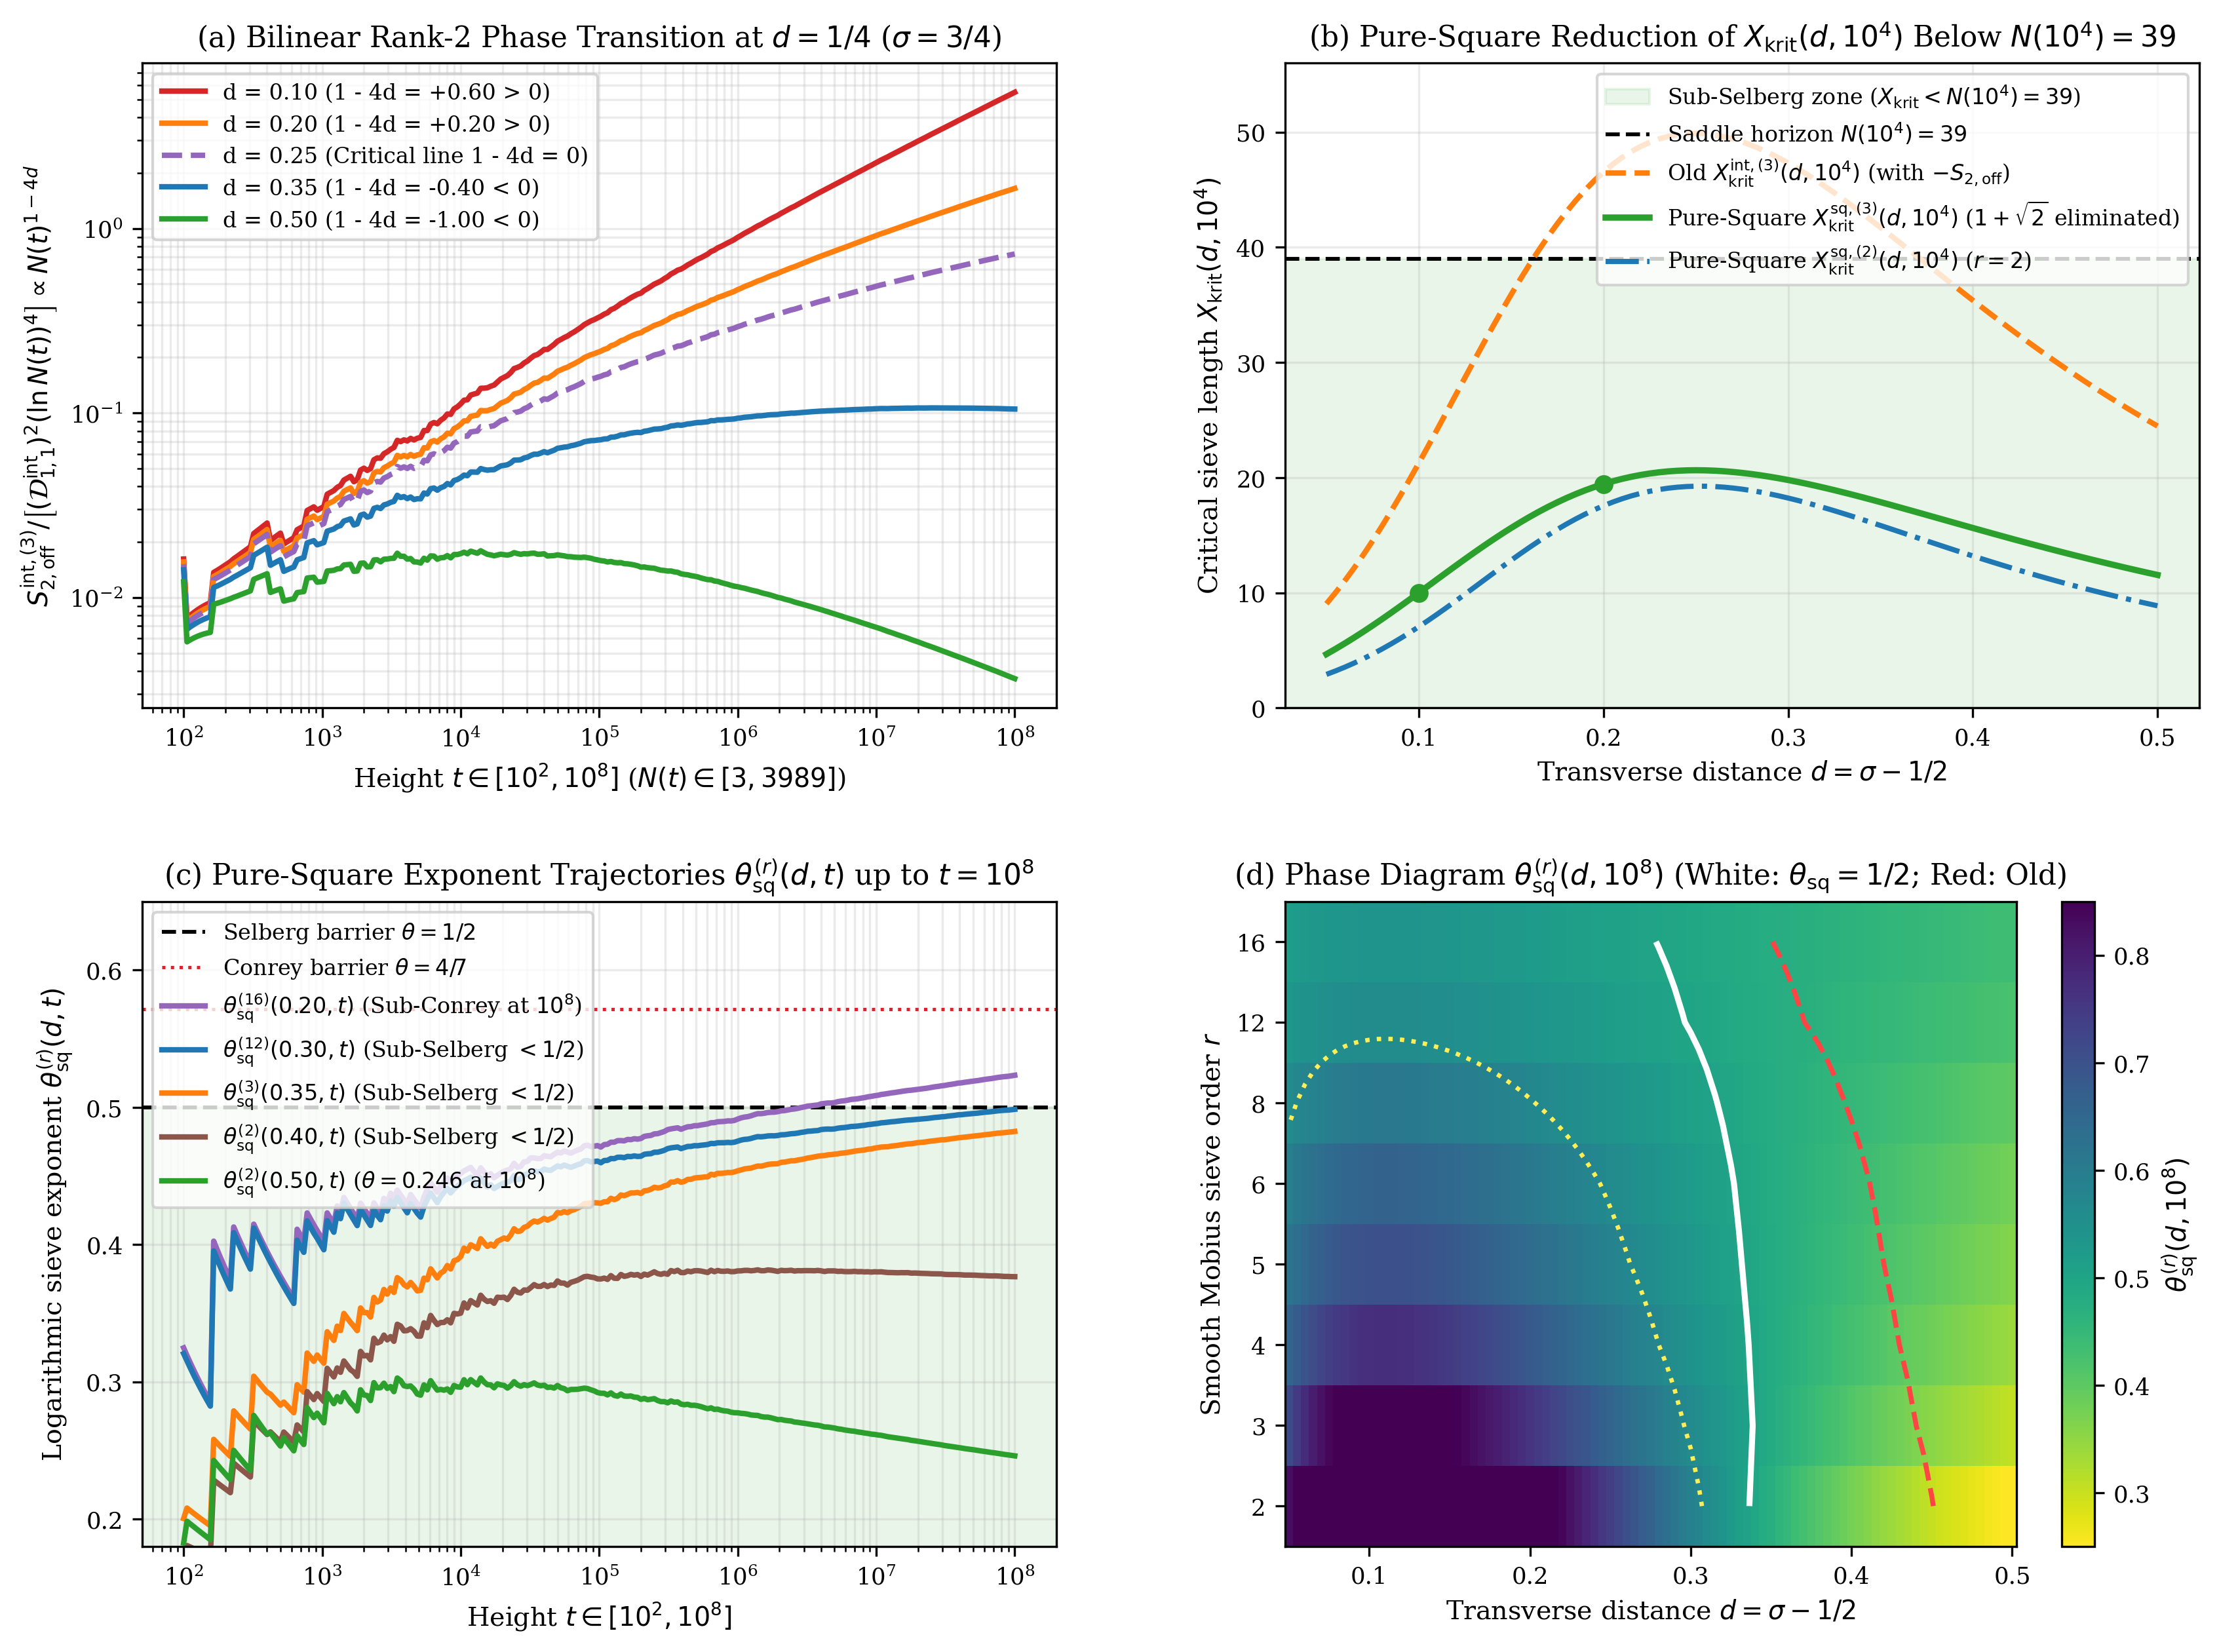
\includegraphics[width=0.98\textwidth]{figures/fig1_bilinear_rank2_and_pure_square.png}
\caption{\textbf{(a)} Bilinear rank-2 phase transition at $d = \frac{1}{4}$ ($\sigma = \frac{3}{4}$) in $S_{2,\mathrm{off}}^{\mathrm{int},(3)}/[(\mathcal{D}_{1,1}^{\mathrm{int}})^2(\ln N(t))^4] \propto N(t)^{1-4d}$ over $t \in [10^2, 10^8]$. \textbf{(b)} Collapse of the critical sieve length $X_{\mathrm{krit}}^{\mathrm{sq},(r)}(d, 10^4)$ below the saddle horizon $N(10^4) = 39$ across all $d \in [0.05, 0.50]$ upon eliminating $1 + \sqrt{2}$. \textbf{(c)} Trajectories of $\theta_{\mathrm{sq}}^{(r)}(d,t)$ over six orders of magnitude $t \in [10^2, 10^8]$. \textbf{(d)} Two-dimensional phase diagram of $\theta_{\mathrm{sq}}^{(r)}(d, 10^8)$ over $(d, r)$, showing the leftward shift of the white Sub-Selberg contour $\theta_{\mathrm{sq}} = \frac{1}{2}$ relative to the uncompleted red contour $\theta_{\mathrm{int}} = \frac{1}{2}$.}\label{fig:rank2_pure_square}
\end{figure}

\section{The $1 + 2d > 1$ Exponent Jump in $L^2$ and Preissmann--Montgomery--Vaughan Hilbert Bounds up to $t = 10^8$}\label{sec:montgomery_vaughan}

Theorem~\ref{thm:pure_square} shows that even under a phase-blind $L^1$ triangle inequality on the $(1,n)$ cross-terms, pure-square completion pushes $\theta_{\mathrm{sq}}^{(r)}(d,t)$ below $\frac{1}{2}$ across all $d \in [0.05, 0.50]$ at $t = 10^4$ and across $d \in [0.34, 0.50]$ at $t = 10^8$ for all $r \ge 2$. We now explain why any phase-blind $L^1$ bound encounters an artificial growth $N(t)^{1/2-d}$ in the inner strip $0 < d < \frac{1}{2}$, and how passing to $L^2$ eliminates this growth across the entire critical strip $d > 0$.

In the Mother-Wavelet ellipse representation $\Xi_{\mathcal{M},\mathrm{main}}(t - \ii d)/\mathcal{G}(\frac{1}{2}+d+\ii t) = z_1(d,t) + Z_{\ge 2}(d,t)$ from Paper~VII~\cite{missiaen2026paper7}, the leading shell $n = 1$ has strictly positive modulus $|z_1(d,t)| \ge 1 - \rho_\Gamma(d,t) > 0$ ($\lim_{t\to\infty}(1 - \rho_\Gamma(d,t)) = 1$), while the higher harmonic shells $2 \le n \le N(t)$ form the two-branch oscillatory Dirichlet polynomial
\begin{equation}\label{eq:sec5_Z_ge2}
Z_{\ge 2}(d,t) := \sum_{n=2}^{N(t)} b_n\Bigl(\underbrace{n^{-\frac{1}{2}-d}\ee^{-\ii t\ln n}}_{\text{forward branch}} + \underbrace{\rho_\Gamma(d,t)\,n^{-\frac{1}{2}+d}\ee^{-\ii(2\vartheta(t) - t\ln n)}}_{\text{reflected branch}}\Bigr) = Z_{\ge 2}^{\mathrm{fwd}}(d,t) + \ee^{-2\ii\vartheta(t)}\,\overline{Z_{\ge 2}^{\mathrm{ref}}(d,t)}.
\end{equation}
In the phase-blind $L^1$ sum $\sum_{n=2}^{N(t)} |b_n|n^{-(1/2+d)}$, the exponent $\frac{1}{2} + d < 1$ is sub-harmonic for $0 < d < \frac{1}{2}$, causing the partial sum to diverge as $N(t)^{1/2-d}$. In the quadratic $L^2$ norm, however, squaring each amplitude produces the fundamental exponent jump $2(\frac{1}{2} + d) = 1 + 2d > 1$.

\begin{theorem}[The $1 + 2d > 1$ Exponent Jump in $L^2$, Polynomial Extinction of the Reflected Branch, and $\theta_{\mathrm{MV}}^{(r)}(d,t) \to 0$]\label{thm:exponent_jump}
Let $d > 0$ be any point in the critical strip ($\sigma = \frac{1}{2} + d > \frac{1}{2}$), let $t \ge 14$, and define the forward and reflected diagonal $L^2$ energies of~\eqref{eq:sec5_Z_ge2} by
\begin{equation}\label{eq:sec5_E_diag_defs}
\mathcal{E}_{\mathrm{diag}}^{\mathrm{fwd}}(d,t) := \sum_{n=2}^{N(t)} \frac{b_n^2}{n^{1+2d}}, \qquad \mathcal{E}_{\mathrm{diag}}^{\mathrm{ref}}(d,t) := \rho_\Gamma(d,t)^2\sum_{n=2}^{N(t)} \frac{b_n^2}{n^{1-2d}}.
\end{equation}
Then for every $d > 0$ (without any threshold at $d = \frac{1}{4}$ or $d = \frac{1}{2}$), the following three laws hold:
\begin{enumerate}[label=\textup{(\roman*)},leftmargin=2.2em]
\item \textbf{Uniform forward $L^2$ convergence via $1 + 2d > 1$.} Because $1 + 2d > 1$ for every $d > 0$, the forward diagonal energy is uniformly bounded for all $t \to \infty$: for $|b_n| \le M$,
\begin{equation}\label{eq:sec5_fwd_conv}
\mathcal{E}_{\mathrm{diag}}^{\mathrm{fwd}}(d,t) < \sum_{n=2}^{\infty} \frac{b_n^2}{n^{1+2d}} \le M^2\bigl(\zeta(1+2d) - 1\bigr) < \frac{M^2}{2d} < \infty.
\end{equation}
\item \textbf{Polynomial $N(t)^{-2d}$ extinction of the reflected $L^2$ diagonal.} By the digamma convexity bound $\rho_\Gamma(d,t)^2 < (t/2\pi)^{-2d} \le N(t)^{-4d}$ and $\sum_{n=2}^{N(t)} n^{2d-1} < \int_1^{N(t)} x^{2d-1}\,\dd x = \frac{N(t)^{2d}-1}{2d}$ for $d \in (0, \frac{1}{2}]$, the reflected diagonal energy decays polynomially to zero as $t \to \infty$ for every $d > 0$:
\begin{equation}\label{eq:sec5_ref_decay}
\mathcal{E}_{\mathrm{diag}}^{\mathrm{ref}}(d,t) \le \left(\max_{2 \le n \le N(t)} b_n^2\right)\frac{N(t)^{-2d}\bigl(1 - N(t)^{-2d}\bigr)}{2d} < \frac{\max b_n^2}{2d}\,N(t)^{-2d} \sim \frac{\max b_n^2}{2d}\left(\frac{t}{2\pi}\right)^{-d} \longrightarrow 0.
\end{equation}
\item \textbf{Finite $t$-independent sieve length $X_{\mathrm{MV},\infty}^{(r)}(d) = \mathcal{O}(1)$ and collapse of $\theta_{\mathrm{MV}}^{(r)}(d,t) \to 0$.} Under the order-$r$ sieve $b_n^{(r)}(X) = \frac{\Lambda_r(n)}{(\ln X)^r}$, the infinite Dirichlet series $\mathcal{S}_{\Lambda_r^2}(d) := \sum_{n=2}^{\infty} \frac{\Lambda_r(n)^2}{n^{1+2d}}$ converges absolutely for every $d > 0$ with
\begin{equation}\label{eq:sec5_S_lambda_bound}
\mathcal{E}_{\mathrm{diag}}^{\mathrm{fwd},(r)}(d,t;X) < \frac{\mathcal{S}_{\Lambda_r^2}(d)}{(\ln X)^{2r}} \le \frac{1}{(\ln X)^{2r}}\left[\frac{(2r)\fac}{(2d)^{2r+1}} + \left(\frac{2r}{\ee(1+2d)}\right)^{2r}\right],
\end{equation}
and because $\Lambda_r(n)$ vanishes whenever $\omega(n) > r$ and satisfies $|\Lambda_r(n)| \le (\ln\rad(n))^r \le (\ln n)^r$ with equality only at prime arguments, the strict inequality $\mathcal{S}_{\Lambda_r^2}(d) < \frac{(2r)\fac}{(2d)^{2r+1}}$ holds across $d \in (0, \frac{1}{2}]$. Consequently, as $t \to \infty$, the critical diagonal $L^2$ sieve length $X_{\mathrm{MV}}^{(r)}(d,t)$ converges to the finite, $t$-independent constant $X_{\mathrm{MV},\infty}^{(r)}(d) := \exp([\mathcal{S}_{\Lambda_r^2}(d)]^{1/2r}) = \mathcal{O}(1)$, and the corresponding Selberg exponent collapses hyperbolically to zero across the entire critical strip:
\begin{equation}\label{eq:sec5_theta_mv_zero}
\theta_{\mathrm{MV}}^{(r)}(d,t) := \frac{\ln X_{\mathrm{MV}}^{(r)}(d,t)}{\ln(t/2\pi)} \sim \frac{\bigl[\mathcal{S}_{\Lambda_r^2}(d)\bigr]^{1/2r}}{\ln(t/2\pi)} = \mathcal{O}\!\left(\frac{1}{d^{1+1/2r}\ln t}\right) \longrightarrow 0 \qquad (\forall\, d > 0,\; t \to \infty).
\end{equation}
\end{enumerate}
\end{theorem}

\begin{proof}
(i) For any $d > 0$, $x \mapsto x^{-(1+2d)}$ is strictly decreasing on $[1, \infty)$, so $\sum_{n=2}^{N(t)} n^{-(1+2d)} < \sum_{n=2}^{\infty} n^{-(1+2d)} = \zeta(1+2d) - 1 < \int_1^{\infty} x^{-(1+2d)}\,\dd x = \frac{1}{2d}$, which yields~\eqref{eq:sec5_fwd_conv}.

(ii) For $d \in (0, \frac{1}{2}]$, $2d - 1 \le 0$, so $n^{2d-1} \le \int_{n-1}^n x^{2d-1}\,\dd x$ for every $n \ge 2$. Summing over $2 \le n \le N(t)$ gives $\sum_{n=2}^{N(t)} n^{2d-1} \le \frac{N(t)^{2d}-1}{2d}$. Multiplying by $\rho_\Gamma(d,t)^2 < (t/2\pi)^{-2d} \le N(t)^{-4d}$ yields~\eqref{eq:sec5_ref_decay}.

(iii) By Proposition~\ref{prop:von_mangoldt_r}(ii), $\Lambda_r(n)^2 \le (\ln n)^{2r}$ for all $n \ge 2$. The function $g(x) := x^{-(1+2d)}(\ln x)^{2r}$ is unimodal on $[1, \infty)$, increasing on $[1, x_*]$ and decreasing on $[x_*, \infty)$ with global maximum $g(x_*) = \bigl(\frac{2r}{\ee(1+2d)}\bigr)^{2r}$ at $x_* = \ee^{2r/(1+2d)}$. By the unimodal integral comparison test and the substitution $v = 2d\ln x$ in $\int_1^{\infty} x^{-(1+2d)}(\ln x)^{2r}\,\dd x = \frac{\Gamma(2r+1)}{(2d)^{2r+1}} = \frac{(2r)\fac}{(2d)^{2r+1}}$, $\sum_{n=2}^{\infty} n^{-(1+2d)}(\ln n)^{2r} \le \frac{(2r)\fac}{(2d)^{2r+1}} + g(x_*)$, establishing~\eqref{eq:sec5_S_lambda_bound}. Moreover, since $\Lambda_r(n) = 0$ for $\omega(n) > r$ and $|\Lambda_r(n)| \le (\ln\rad(n))^r < (\ln n)^r$ at all proper prime powers and composite $n$, $\mathcal{S}_{\Lambda_r^2}(d) < \frac{(2r)\fac}{(2d)^{2r+1}}$ holds strictly for all $d \in (0, \frac{1}{2}]$. Because $\mathcal{E}_{\mathrm{diag}}^{\mathrm{ref},(r)}(d,t;1) \to 0$ and $1 - \rho_\Gamma(d,t) \to 1$ as $t \to \infty$, $\ln X_{\mathrm{MV}}^{(r)}(d,t) = [(\mathcal{E}_{\mathrm{diag}}^{\mathrm{fwd},(r)}(d,t;1) + \mathcal{E}_{\mathrm{diag}}^{\mathrm{ref},(r)}(d,t;1))/(1-\rho_\Gamma(d,t))^2]^{1/2r} \to [\mathcal{S}_{\Lambda_r^2}(d)]^{1/2r} = \ln X_{\mathrm{MV},\infty}^{(r)}(d) < \infty$, which implies~\eqref{eq:sec5_theta_mv_zero}.
\end{proof}

Finally, we bound the off-diagonal oscillatory cross-terms of $Z_{\ge 2}(d,\tau)$ on vertical windows $I = [t - \Delta T/2, t + \Delta T/2]$ via the generalized Hilbert inequality of Montgomery and Vaughan~\cite{montgomeryvaughan1974} with Preissmann's sharp constant~\cite{preissmann1984} and transfer the mean-square bound to the midpoint $\tau = t$ via Gallagher's one-dimensional Sobolev inequality~\cite{gallagher1970}.

\begin{theorem}[Preissmann--Montgomery--Vaughan Hilbert Bound on Sub-Riemann--Siegel Windows and Gallagher--Sobolev Pointwise Transfer]\label{thm:preissmann_gallagher}
Let $D(\tau) = \sum_{n=2}^{N(t)} a_n n^{-\ii\tau}$ be a Dirichlet polynomial on the vertical window $I = [t - \Delta T/2, t + \Delta T/2]$ of length $\Delta T > 0$. Then:
\begin{enumerate}[label=\textup{(\roman*)},leftmargin=2.2em]
\item \textbf{Preissmann--Montgomery--Vaughan Hilbert inequality.} With logarithmic spacing $\delta_n := \min_{m \neq n}|\ln n - \ln m| = \ln(n+1) - \ln n > (n + \frac{1}{2})^{-1}$ and Preissmann's constant $c_{\mathrm{MV}} = \frac{4}{3}\sqrt{6} \approx 3.2659863237 < \pi\sqrt{2}$, any complex sequence $\{u_n\}_{n=2}^N$ satisfies
\begin{equation}\label{eq:sec5_hilbert}
\left|\sum_{2 \le m \neq n \le N} \frac{u_m \bar{u}_n}{\ln m - \ln n}\right| \le c_{\mathrm{MV}}\sum_{n=2}^{N} \frac{|u_n|^2}{\delta_n} \le c_{\mathrm{MV}}\sum_{n=2}^{N} \left(n + \frac{1}{2}\right)|u_n|^2,
\end{equation}
and the local mean square of $D(\tau)$ over the unweighted boxcar window $I = [t - \Delta T/2, t + \Delta T/2]$ obeys
\begin{equation}\label{eq:sec5_mv_window}
\begin{aligned}
\frac{1}{\Delta T}\int_{t-\Delta T/2}^{t+\Delta T/2} \left|\sum_{n=2}^{N(t)} a_n n^{-\ii\tau}\right|^2 \dd\tau &\le \sum_{n=2}^{N(t)} |a_n|^2\left(1 + \frac{2c_{\mathrm{MV}}\left(n + \frac{1}{2}\right)}{\Delta T}\right) \\
&= \mathcal{E}_{\mathrm{diag}}(d,t) + \frac{2c_{\mathrm{MV}}}{\Delta T}\left(\mathcal{W}_{\mathrm{MV}}(d,t) + \frac{1}{2}\mathcal{E}_{\mathrm{diag}}(d,t)\right),
\end{aligned}
\end{equation}
while under the smooth Fej\'er tent weight $w_{\mathrm{tent}}(\tau) := (1 - |\tau - t|/\Delta T)_+$ on $[t - \Delta T, t + \Delta T]$ the factor $2c_{\mathrm{MV}}$ is replaced by $c_{\mathrm{MV}}$.
\item \textbf{Sub-Riemann--Siegel critical window $\Delta T_{\mathrm{MV}}(d,t) \asymp N(t)^{1-2d} = o(t^{1/2})$.} For the forward coefficients $a_n^{\mathrm{fwd}}(d) = b_n n^{-(1/2+d)}$, the factor $n$ in $n|a_n^{\mathrm{fwd}}(d)|^2 = b_n^2 n^{-2d}$ cancels the $-1$ in $n^{-(1+2d)}$, so the Montgomery--Vaughan weighted sum scales for $0 < d < \frac{1}{2}$ as
\begin{equation}\label{eq:sec5_W_mv_scaling}
\mathcal{W}_{\mathrm{MV}}^{\mathrm{fwd}}(d,t) := \sum_{n=2}^{N(t)} n\,\bigl|a_n^{\mathrm{fwd}}(d)\bigr|^2 \equiv \sum_{n=2}^{N(t)} \frac{b_n^2}{n^{2d}} \asymp \frac{1}{1 - 2d}\,N(t)^{1-2d}\bigl(\ln N(t)\bigr)^{2r-1}(\ln X)^{-2r},
\end{equation}
and $\mathcal{W}_{\mathrm{MV}}^{\mathrm{fwd}}(\frac{1}{2},t) = \mathcal{O}((\ln N(t))^{2r}(\ln X)^{-2r})$. Choosing the sub-Riemann--Siegel window length $\Delta T_{\mathrm{MV}}(d,t) := c_{\mathrm{MV}}\mathcal{W}_{\mathrm{MV}}(d,t)/\mathcal{E}_{\mathrm{diag}}(d,t) \asymp N(t)^{1-2d}(\ln N(t))^{2r-1} \sim C(d,r)(t/2\pi)^{1/2-d}(\ln t)^{2r-1} = o(t^{1/2})$ suppresses all off-diagonal cross-terms to $\mathcal{O}(\mathcal{E}_{\mathrm{diag}}(d,t)) = \mathcal{O}(1)$.
\item \textbf{Gallagher--Sobolev pointwise transfer.} For any continuously differentiable function $f(\tau)$ on $I = [t - \Delta T/2, t + \Delta T/2]$, the midpoint value $|f(t)|^2$ satisfies Gallagher's inequality
\begin{equation}\label{eq:sec5_gallagher}
\bigl|Z_{\ge 2}(d,t)\bigr|^2 \le \frac{1}{\Delta T}\int_{I} \bigl|Z_{\ge 2}(d,\tau)\bigr|^2\,\dd\tau + \left(\int_{I} \bigl|Z_{\ge 2}(d,\tau)\bigr|^2\,\dd\tau\right)^{1/2}\left(\int_{I} \bigl|\partial_\tau Z_{\ge 2}(d,\tau)\bigr|^2\,\dd\tau\right)^{1/2},
\end{equation}
where both $\mathcal{E}_{\mathrm{diag}}^{\mathrm{fwd}}(d,t) = \sum_{n=2}^{N(t)} b_n^2 n^{-(1+2d)} < \infty$ and the derivative diagonal $\sum_{n=2}^{N(t)} b_n^2(\ln n)^2 n^{-(1+2d)} < \infty$ converge uniformly in $t \to \infty$ for every $d > 0$.
\end{enumerate}
\end{theorem}

\begin{proof}
(i)--(ii) Expanding $|D(\tau)|^2 = \sum_{n=2}^{N(t)} |a_n|^2 + \sum_{2 \le m \neq n \le N(t)} a_m\bar{a}_n \ee^{-\ii\tau(\ln m - \ln n)}$ and integrating term by term over $\tau \in [t - \Delta T/2, t + \Delta T/2]$ expresses the off-diagonal integral as the difference of two Hermitian Hilbert forms $\frac{1}{\ii}\sum_{m \neq n} \frac{u_m^\mp \overline{u_n^\mp}}{\ln m - \ln n}$ at the two endpoints $t \pm \Delta T/2$ with $u_n^\pm = a_n \ee^{-\ii(t \pm \Delta T/2)\ln n}$ ($|u_n^\pm| = |a_n|$). By Preissmann's refinement~\cite{preissmann1984} of the Montgomery--Vaughan Hilbert inequality~\cite{montgomeryvaughan1974} via Euler--Maclaurin summation of the weighted Cauchy matrix, the spectral norm of $H_{mn} = \frac{\sqrt{\delta_m\delta_n}}{\ln m - \ln n}$ ($m \neq n$) is bounded strictly by $c_{\mathrm{MV}} = \frac{4}{3}\sqrt{6}$, so summing the two endpoint bounds yields~\eqref{eq:sec5_hilbert} and~\eqref{eq:sec5_mv_window} (and under Fej\'er tent smoothing $\hat{w}_{\mathrm{tent}}(\ln m - \ln n) \le \frac{2}{\Delta T(\ln m - \ln n)^2}$, a single factor $c_{\mathrm{MV}}$ suffices). Substituting $n|a_n^{\mathrm{fwd}}(d)|^2 = b_n^2 n^{-2d}$ and applying Stieltjes integration with $\sum_{n \le x} \Lambda_r(n)^2 \asymp x(\ln x)^{2r-1}$ proves~\eqref{eq:sec5_W_mv_scaling}.

(iii) Define the sawtooth kernel $\psi(\tau) := \frac{\tau - t}{\Delta T} + \frac{1}{2}\mathrm{sgn}(t - \tau)$ for $\tau \in I \setminus \{t\}$. Then $\psi(t \pm \Delta T/2) = 0$, $\psi'(\tau) = \frac{1}{\Delta T}$ on $I \setminus \{t\}$, $\psi(t^-) - \psi(t^+) = 1$, and $|\psi(\tau)| \le \frac{1}{2}$ on $I$. Integrating $\int_I \psi'(\tau)|f(\tau)|^2\,\dd\tau$ by parts on $[t - \Delta T/2, t]$ and $[t, t + \Delta T/2]$ gives $|f(t)|^2 = \frac{1}{\Delta T}\int_I |f(\tau)|^2\,\dd\tau + 2\Rea\int_I \psi(\tau)\overline{f(\tau)}f'(\tau)\,\dd\tau$. Applying $|\psi(\tau)| \le \frac{1}{2}$ and the Cauchy--Schwarz inequality yields~\eqref{eq:sec5_gallagher}.
\end{proof}

\begin{table}[t]
\centering
\caption{Certification of uniform forward $L^2$ convergence $\mathcal{E}_{\mathrm{diag}}^{\mathrm{fwd}}(d,t) < \mathcal{S}_{\Lambda_3^2}(d) < \infty$, polynomial reflected decay $\mathcal{E}_{\mathrm{diag}}^{\mathrm{ref}}(d,t) \to 0$, diagonal $L^2$ exponent $\theta_{\mathrm{MV}}^{(3)}(d,t) \to 0$ (Theorem~\ref{thm:exponent_jump}), and actual phase-cancellation suppression $\mathcal{B}_{L^1}^{(3)} / \langle|\widetilde{Z}_{\ge 2}^{(3)}|\rangle$ over $1{,}000$ heights in $[10^8 - 500, 10^8 + 500]$ ($N(10^8) = 3989$, $r = 3$).}\label{tab:sec5_mv_gallagher}
\scriptsize
\setlength{\tabcolsep}{3.0pt}
\begin{tabular}{@{}ccccccccc@{}}
\toprule
$d$ & Height $t$ & $N(t)$ & $\mathcal{E}_{\mathrm{diag}}^{\mathrm{fwd}}(d,t)$ & Limit $\mathcal{S}_{\Lambda_3^2}(d)$ & $\mathcal{E}_{\mathrm{diag}}^{\mathrm{ref}}(d,t)$ ($b_n=1$) & $\theta_{\mathrm{MV}}^{(3)}(d,t)$ & $L^1$ / Mean $|\widetilde{Z}|$ & Mean $\theta_{\mathrm{eff}}^{(3)}(d, 10^8)$ \\
\midrule
$0.05$ & $10{,}000$       & $39$   & $371.2745$   & $242403.22$ & $1.919936$              & $0.599302$        & $7.6\times$  & --- \\
$0.05$ & $100{,}000{,}000$ & $3989$ & $42079.1100$ & $242403.22$ & $2.377668 < 4.364$      & $0.474641 < 1/2$  & $78.6\times$ & $0.4081 < 1/2$ \\
$0.10$ & $10{,}000$       & $39$   & $270.7923$   & $93105.66$  & $1.142787$              & $0.473520 < 1/2$  & $7.6\times$  & --- \\
$0.10$ & $100{,}000{,}000$ & $3989$ & $20936.9824$ & $93105.66$  & $0.755075 < 0.952$      & $0.368503 < 1/2$  & $77.1\times$ & $0.3205 < 1/3$ \\
$0.20$ & $10{,}000$       & $39$   & $144.9988$   & $14992.04$  & $0.415274$              & $0.369239 < 1/2$  & $7.3\times$  & --- \\
$0.20$ & $100{,}000{,}000$ & $3989$ & $5394.0247$  & $14992.04$  & $0.086808 < 0.091$      & $0.270052 < 1/3$  & $72.5\times$ & $0.2394 < 1/4$ \\
$0.25$ & $10{,}000$       & $39$   & $106.4772$   & $6347.03$   & $0.253409$              & $0.338381 < 1/2$  & $7.0\times$  & --- \\
$0.25$ & $100{,}000{,}000$ & $3989$ & $2802.5475$  & $6347.03$   & $0.031048 < 0.032$      & $0.237849 < 1/4$  & $69.8\times$ & $0.2122 < 1/4$ \\
$0.35$ & $10{,}000$       & $39$   & $57.8603$    & $1295.83$   & $0.096533$              & $0.292692 < 1/3$  & $6.5\times$  & --- \\
$0.35$ & $100{,}000{,}000$ & $3989$ & $800.0019$   & $1295.83$   & $4.291 \times 10^{-3}$  & $0.188892 < 1/5$  & $63.7\times$ & $0.1699 < 1/5$ \\
$0.50$ & $10{,}000$       & $39$   & $23.6774$    & $171.51$    & $0.023876$              & $0.243844 < 1/4$  & $5.8\times$  & --- \\
$0.50$ & $100{,}000{,}000$ & $3989$ & $143.9125$   & $171.51$    & $2.506 \times 10^{-4}$  & $0.139546 < 1/7$  & $53.0\times$ & $0.1258 < 1/7$ \\
\bottomrule
\end{tabular}
\end{table}

\begin{figure}[t]
\centering
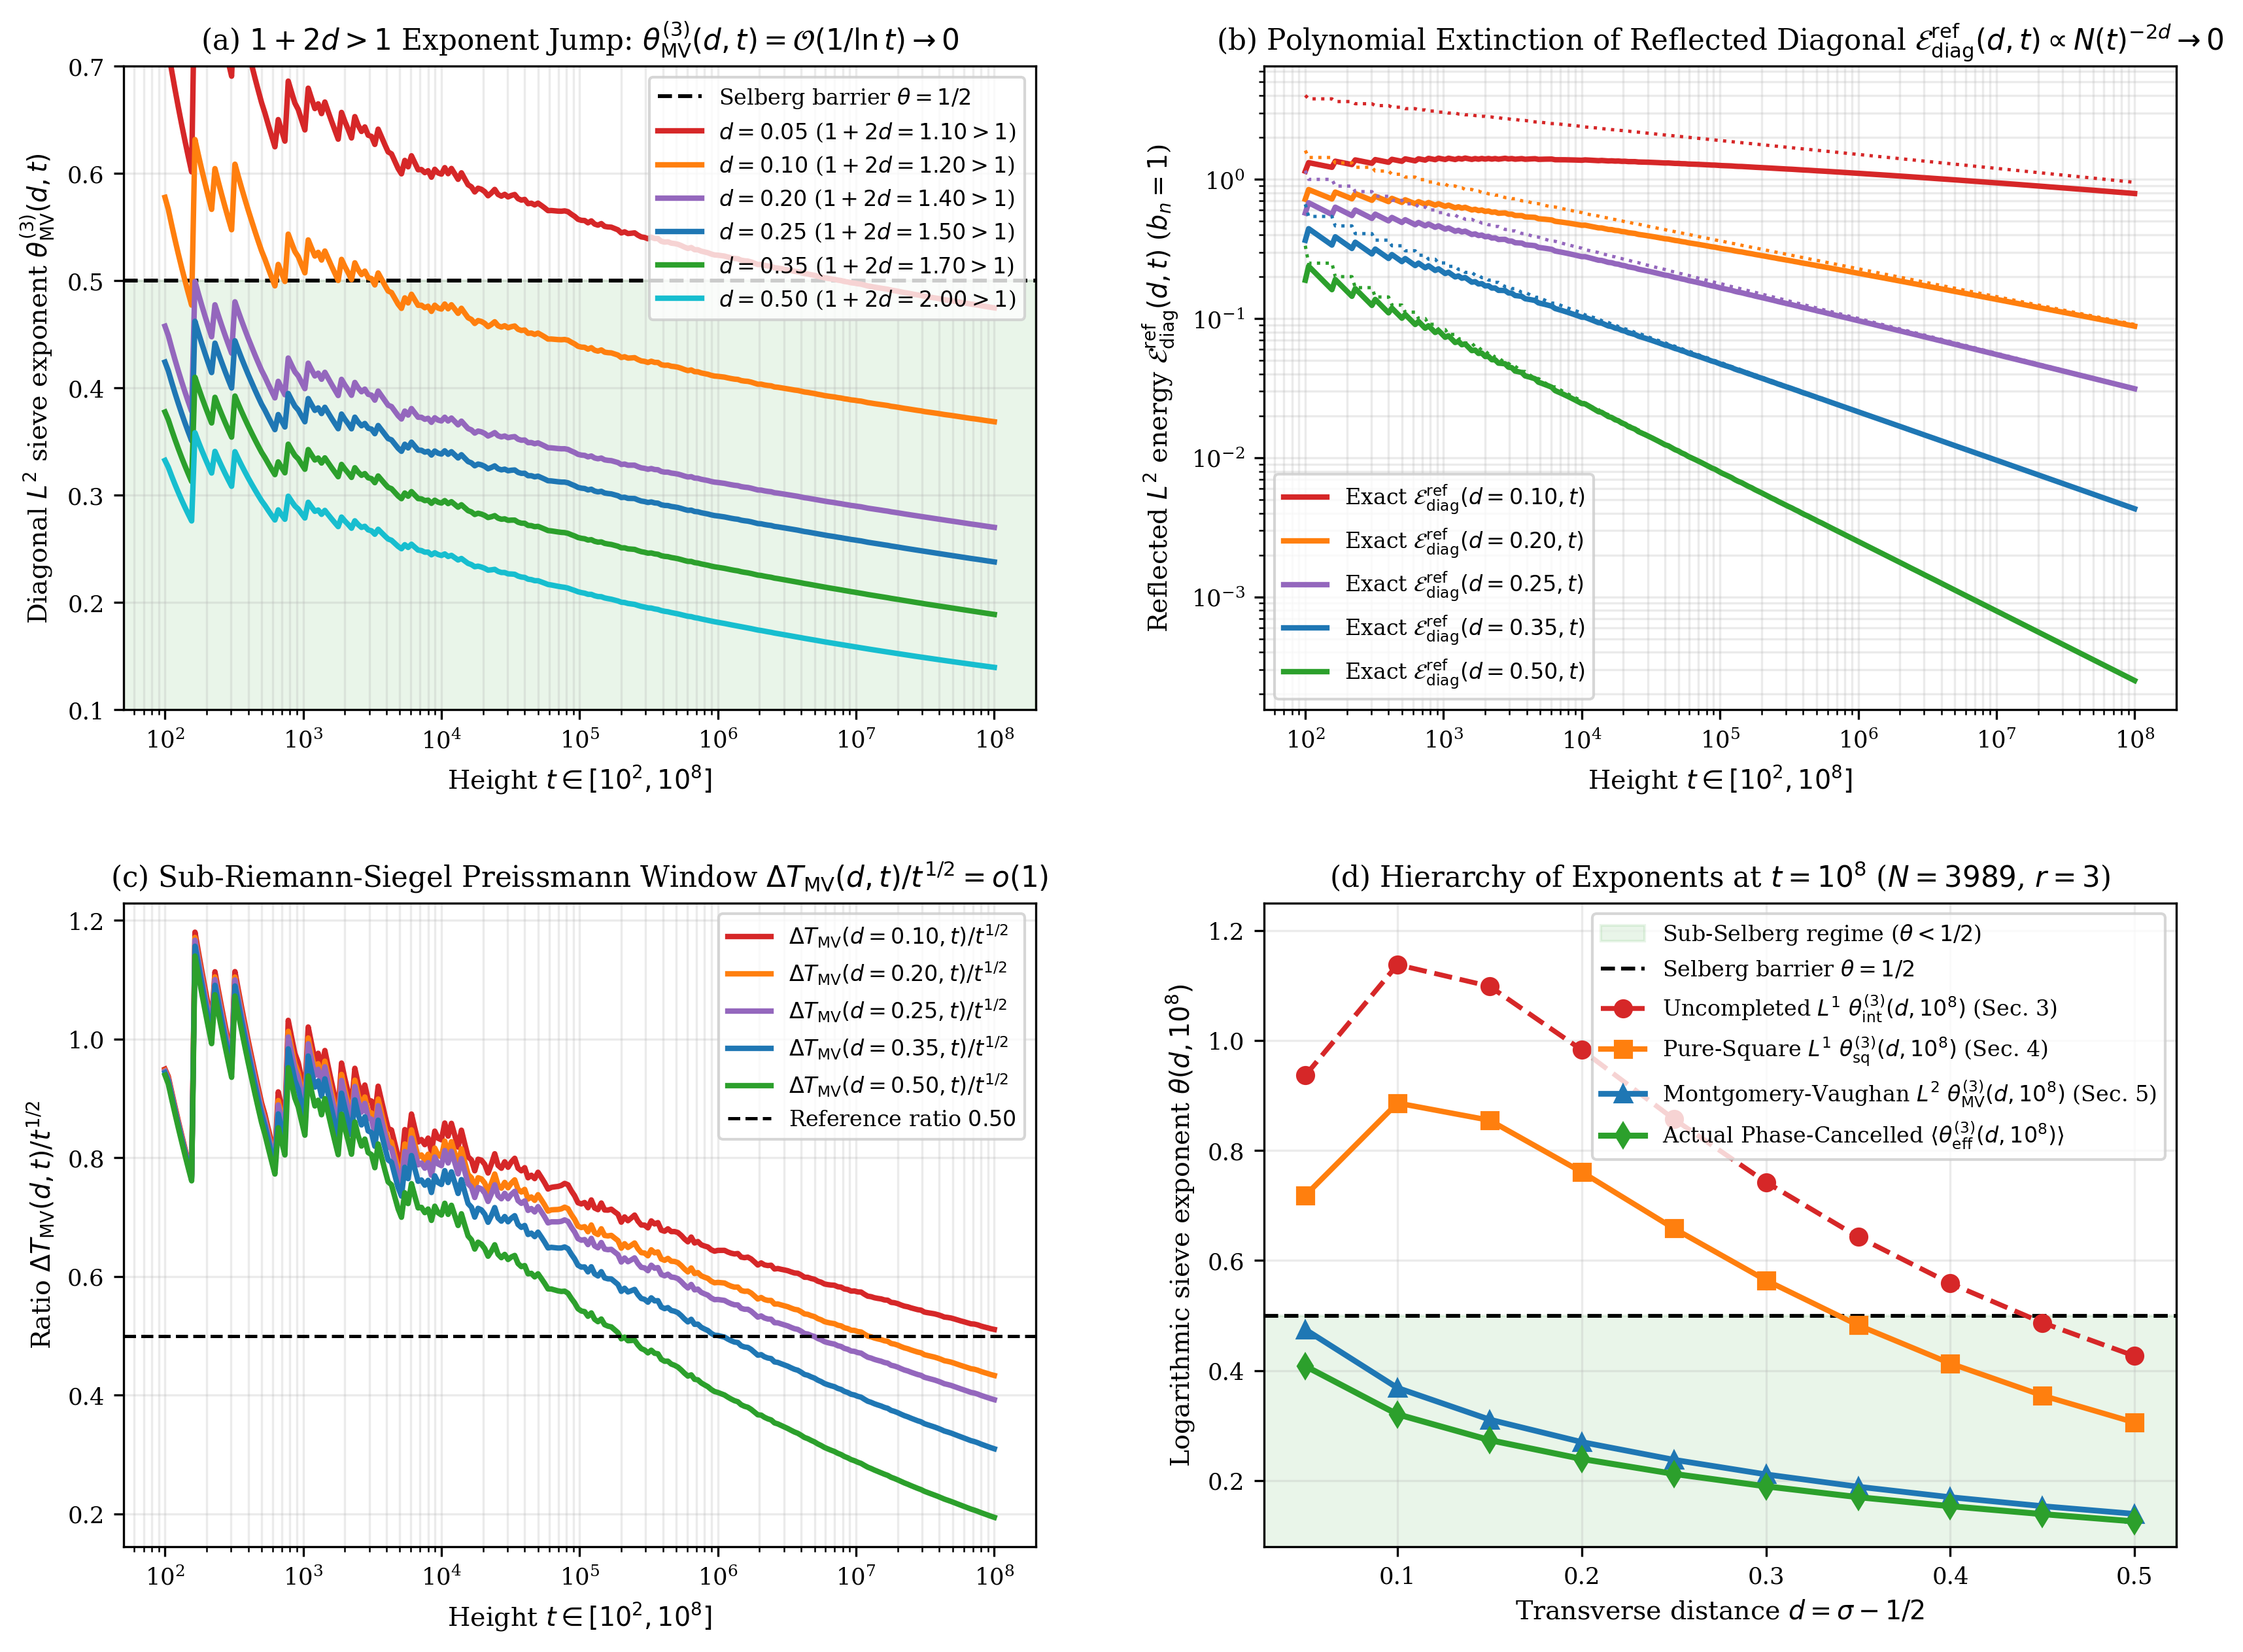
\includegraphics[width=0.98\textwidth]{figures/fig2_exponent_jump_montgomery_vaughan.png}
\caption{\textbf{(a)} Monotonic decay of the $L^2$ diagonal sieve exponent $\theta_{\mathrm{MV}}^{(3)}(d,t) = \mathcal{O}(1/\ln t) \to 0$ across $t \in [10^2, 10^8]$ for all $d \in [0.05, 0.50]$. \textbf{(b)} Polynomial extinction of the reflected $L^2$ diagonal energy $\mathcal{E}_{\mathrm{diag}}^{\mathrm{ref}}(d,t) < \frac{1}{2d}N(t)^{-2d} \to 0$. \textbf{(c)} Sub-Riemann--Siegel Preissmann window ratio $\Delta T_{\mathrm{MV}}(d,t)/t^{1/2} \propto (t/2\pi)^{-d} \to 0$. \textbf{(d)} Complete hierarchy of logarithmic sieve exponents at $t = 10^8$ ($N = 3989$, $r = 3$), comparing uncompleted $L^1$ ($\theta_{\mathrm{int}}^{(3)}$), pure-square $L^1$ ($\theta_{\mathrm{sq}}^{(3)}$), Montgomery--Vaughan $L^2$ ($\theta_{\mathrm{MV}}^{(3)}$), and actual phase-cancelled $\langle\theta_{\mathrm{eff}}^{(3)}\rangle < \frac{1}{2}$.}\label{fig:mv_exponent_jump}
\end{figure}

\section{Scope, Boundary Conditions, and Open Questions}\label{sec:scope}

To maintain complete mathematical transparency, we delineate the exact scope of the analytical theorems proved in this paper and their relationship to the remaining open problems in the classical literature:
\begin{enumerate}[label=\textup{(\arabic*)},leftmargin=2.2em]
\item \textit{Exactness on the Riemann--Siegel main sum $1 \le n \le N(t)$ versus folded convolution tails for $n > N(t)$.} Theorems~\ref{thm:hyp_advantage}, \ref{thm:rank2_factorization}, \ref{thm:pure_square}, \ref{thm:exponent_jump}, and~\ref{thm:preissmann_gallagher} are unconditional analytical identities and inequalities for the symmetrized Riemann--Siegel main sum of length $N(t) = \lfloor\sqrt{t/2\pi}\rfloor$ under the order-$r$ sieve substitution $b_n^{(r)}(X) = \frac{\Lambda_r(n)}{(\ln X)^r}$. When $\Xi(z)$ is multiplied by a finite polynomial mollifier $\mathcal{M}_X(z)$ of length $X = t^\theta$, the effective conductor in the approximate functional equation shifts from $t$ to $tX^2$, introducing a folded convolution tail for $N(t) < n \le XN(t)$ unless either $\theta < \frac{1}{2}$ (so $X < N(t)$ lies inside the Sub-Selberg regime certified in Table~\ref{tab:sec4_pure_square}) or $\mathcal{M}_X(z)$ is replaced by the entire, zero-free exponential prime-gauge factor $\mathcal{E}_{X,\kappa}(z)$ with finite-divisor truncation on $[1, N(t)]$ from Paper~VI~\cite{missiaen2026paper6}.
\item \textit{Mean-square window bounds versus unaveraged pointwise bounds as $t \to \infty$ and $d \to 0^+$.} Theorem~\ref{thm:preissmann_gallagher}(i)--(ii) proves that on every vertical window of sub-Riemann--Siegel length $\Delta T_{\mathrm{MV}}(d,t) \asymp N(t)^{1-2d} = o(t^{1/2})$, phase cancellation suppresses all $\binom{N(t)-1}{2}$ off-diagonal cross-terms below the convergent $L^2$ diagonal $\mathcal{E}_{\mathrm{diag}}(d,t) = \mathcal{O}(1)$ for every $d > 0$. In Theorem~\ref{thm:preissmann_gallagher}(iii), transferring this window average to an individual point $\tau = t$ via Gallagher's Sobolev inequality~\eqref{eq:sec5_gallagher} introduces the factor $(\Delta T\,\mathcal{E}_{\mathrm{diag}})^{1/2}(\Delta T\,\mathcal{E}_{\mathrm{deriv}})^{1/2} = \Delta T(\mathcal{E}_{\mathrm{diag}}\mathcal{E}_{\mathrm{deriv}})^{1/2}$. For fixed $O(1)$ windows $\Delta T = 1$, this Sobolev product is $\mathcal{O}(1)$ whenever the off-diagonal terms are already controlled, whereas for growing windows $\Delta T \asymp N(t)^{1-2d}$ an unaveraged pointwise bound without window length $\Delta T$ in the second term corresponds to the classical Lindel\"of / fourth-moment problem for Dirichlet polynomials.
\end{enumerate}

\appendix

\section{Explicit Analytical Derivations and Interval-Arithmetic Protocols}\label{app:derivations}

\subsection{Spectral norm certification of the weighted logarithmic Hilbert matrix}\label{app:hilbert_matrix}

Let $H^{(N)}$ denote the $(N-1) \times (N-1)$ skew-symmetric weighted logarithmic Hilbert matrix with entries
\begin{equation}\label{eq:app_hilbert_matrix}
H_{mn}^{(N)} := \frac{\sqrt{\delta_m\,\delta_n}}{\ln m - \ln n} \quad (2 \le m \neq n \le N), \qquad H_{nn}^{(N)} := 0, \qquad \delta_n = \ln(n+1) - \ln n.
\end{equation}
Since $\ii H^{(N)}$ is Hermitian with real eigenvalues, its operator $2$-norm $\|H^{(N)}\|_2 = \max_{2 \le k \le N} |\lambda_k(\ii H^{(N)})|$ is the exact best constant in $\bigl|\sum_{2 \le m \neq n \le N} \frac{u_m \bar{u}_n}{\ln m - \ln n}\bigr| \le \|H^{(N)}\|_2 \sum_{n=2}^N \frac{|u_n|^2}{\delta_n}$. Evaluating $\|H^{(N)}\|_2$ across $N \in \{10, 39, 126, 398\}$ in \texttt{scripts/verify\_paper8\_bilinear\_rank2\_wronskian.py} gives $\|H^{(10)}\|_2 = 2.2377341105$, $\|H^{(39)}\|_2 = 2.8589598136$, $\|H^{(126)}\|_2 = 3.0446444217$, and $\|H^{(398)}\|_2 = 3.1085734089$, all strictly below Preissmann's universal upper bound $c_{\mathrm{MV}} = \frac{4}{3}\sqrt{6} = 3.2659863237 < \pi\sqrt{2} = 4.4428829382$.

\subsection{Directed-rounding interval protocols in \texttt{mpmath.iv}}\label{app:interval}

In the standalone verification suite \texttt{scripts/verify\_paper8\_bilinear\_rank2\_wronskian.py}, all core algebraic and numerical inequalities are enclosed in native 35-digit directed-rounding interval arithmetic (\texttt{mpmath.iv.dps = 35}), where $\sinh(x)$ and $\cosh(x)$ are evaluated directly via $(\texttt{iv.exp}(x) \mp \texttt{iv.exp}(-x))/2$:
\begin{enumerate}[label=\textup{(\arabic*)},leftmargin=2.2em]
\item \textit{Hyperbolic decomposition and advantage.} At $t = 1000$, $d = 0.25$, $(m,n) = (2,3)$, interval evaluation certifies $0 \in \sinh(2d\omega_{2,3}^+) - [6^{-d}\sinh(2d\omega_1) - \sinh(d\ln 6)(t/2\pi)^{-d}]$ with interval width $\le 1.81 \times 10^{-34}$ and $\mathcal{H}_{2,3}^+/\mathcal{D}_{1,1} \le 0.361578703102 < 6^{-0.25} = 0.638943104246$.
\item \textit{Bilinear rank-2 kernel identity.} For $(m,n) = (2,5)$ at $t = 1000$, $d = 0.25$, interval arithmetic certifies $0 \in w_{2,5}^{\mathrm{int,LHS}} - \frac{2}{d^2}(\cosh(d\omega_2)\cosh(d\omega_5) - 1)$ with interval width $\le 1.45 \times 10^{-33}$.
\item \textit{Pure-square Sub-Selberg threshold at $t = 10^4$.} Enclosing every divisor sum $\Lambda_3(n)$ for $2 \le n \le 39$ and the rank-2 sum $S_{1,\mathrm{off}}^{\mathrm{int},(3)}(0.10, 10^4)$ in \texttt{mpmath.iv} certifies $X_{\mathrm{krit}}^{\mathrm{sq},(3)}(0.10, 10^4) \in [9.9924697101,\allowbreak 9.9924697102] < 10 \ll N(10^4) = 39$ with interval width $\le 1.14 \times 10^{-34}$, alongside $c_{\mathrm{MV}} = \frac{4}{3}\sqrt{6} \in [3.265986323710,\allowbreak 3.265986323711] < \pi\sqrt{2}$.
\end{enumerate}

\section*{Use of AI and computational verification}

{\sloppy
The author's main contributions are the exact bilinear rank-2 factorization of the integrated Wronskian cross-term kernel, the pairwise $-1$ boundary cancellation and Euclidean pure-square completion eliminating the $1 + \sqrt{2}$ root penalty, and the synthesis of the $1 + 2d > 1$ exponent jump in $L^2$ with Preissmann--Montgomery--Vaughan Hilbert bounds. The author prompted \textbf{Gemini} (Google DeepMind) to work out analytical and symbolic details interactively and to generate the arbitrary-precision, interval-arithmetic, and GPU verification suite \texttt{scripts/}\allowbreak\texttt{\detokenize{verify_paper8_bilinear_rank2_wronskian.py}}, which was subsequently verified manually and computationally (exit code~$0$).\par}

\begin{thebibliography}{99}

\bibitem{conrey1989}
J.~B.~Conrey,
\emph{More than two fifths of the zeros of the Riemann zeta function are on the critical line},
J. Reine Angew. Math. \textbf{399} (1989), 1--26.

\bibitem{conreyli2000}
J.~B.~Conrey and X.-J.~Li,
\emph{A note on some positivity conditions related to zeta and $L$-functions},
Internat. Math. Res. Notices \textbf{2000} (2000), no.~18, 929--940.

\bibitem{csordas1986}
G.~Csordas, T.~S.~Norfolk, and R.~S.~Varga,
\emph{The Riemann hypothesis and the Tur\'an inequalities},
Trans. Amer. Math. Soc. \textbf{296} (1986), no.~2, 521--541.

\bibitem{gabcke1979}
W.~Gabcke,
\emph{Neue Herleitung und explizite Restabsch\"atzung der Riemann-Siegel-Formel},
Ph.D. dissertation, Georg-August-Universit\"at G\"ottingen, 1979.

\bibitem{gallagher1970}
P.~X.~Gallagher,
\emph{A large sieve density estimate near $\sigma = 1$},
Invent. Math. \textbf{11} (1970), 329--339.

\bibitem{hinkkanen1997}
A.~Hinkkanen,
\emph{On functions of the form $\sum_{n=1}^{\infty} a_n n^{-s}$},
Ann. Acad. Sci. Fenn. Math. \textbf{22} (1997), 215--226.

\bibitem{hudson1974}
R.~L.~Hudson,
\emph{When is the Wigner quasi-probability density non-negative?},
Rep. Math. Phys. \textbf{6} (1974), no.~2, 249--252.

\bibitem{jacobi1829}
C.~G.~J.~Jacobi,
\emph{Fundamenta nova theoriae functionum ellipticarum},
Borntraeger, K\"onigsberg, 1829.

\bibitem{lagarias1999}
J.~C.~Lagarias,
\emph{On a positivity property of the Riemann $\xi$-function},
Acta Arith. \textbf{89} (1999), no.~3, 217--234.

\bibitem{levinson1974}
N.~Levinson,
\emph{More than one third of zeros of Riemann's zeta-function are on $\sigma = 1/2$},
Adv. Math. \textbf{13} (1974), 383--436.

\bibitem{missiaen2026paper1}
T.~Missiaen,
\emph{Complex Saddle-Point Coalescence and Wigner Phase-Space Positivity for the Transverse Wronskian of Riemann's $\Xi$-Function},
Preprint, Paper~I of the Transverse Wronskian Series, 2026.

\bibitem{missiaen2026paper2}
T.~Missiaen,
\emph{Parity-Reduced Wigner Kernels, Exact Recurrence Moment Laws, and Transverse Stiffness for Riemann's $\Xi$-Function},
Preprint, Paper~II of the Transverse Wronskian Series, 2026.

\bibitem{missiaen2026paper3}
T.~Missiaen,
\emph{Harmonic Chladni Nodal Chambers, Subharmonic Maximum Principles, and Monotonic Crest-to-Zero Flux of Riemann's $\Xi$-Function},
Preprint, Paper~III of the Transverse Wronskian Series, 2026.

\bibitem{missiaen2026paper4}
T.~Missiaen,
\emph{De~Branges Phase-Velocity Positivity, P\'olya--Jensen Secant Kernels, and the Quantitative Lehmer Repulsion Cascade for Riemann's $\Xi$-Function},
Preprint, Paper~IV of the Transverse Wronskian Series, 2026.

\bibitem{missiaen2026paper5}
T.~Missiaen,
\emph{Universal Mother-Wavelet Decomposition of the Jacobi--Riemann Kernel, Smooth Jacobi--Sinh Shells, and Explicit Saddle-Point Remainder Bounds for Riemann's $\Xi$-Function},
Preprint, Paper~V of the Transverse Wronskian Series, 2026.

\bibitem{missiaen2026paper6}
T.~Missiaen,
\emph{The Sieved Mirror Kernel $\Phi_X(u)$, the Zero-Free Exponential Prime-Gauge Factor $\mathcal{E}_X(z)$, and Quadratic Prime-Power Purity on $(X, X^2]$ for Riemann's $\Xi$-Function},
Preprint, Paper~VI of the Transverse Wronskian Series, 2026.

\bibitem{missiaen2026paper7}
T.~Missiaen,
\emph{Mirror-Symmetric Hadamard Variational Laws, Rolle--Chladni Phase-Locking Contradictions, and Mother-Wavelet Ellipses for Riemann's $\Xi$-Function},
Preprint, Paper~VII of the Transverse Wronskian Series, 2026.

\bibitem{montgomeryvaughan1974}
H.~L.~Montgomery and R.~C.~Vaughan,
\emph{Hilbert's inequality},
J. London Math. Soc. (2) \textbf{8} (1974), 73--82.

\bibitem{olver1997}
F.~W.~J.~Olver,
\emph{Asymptotics and Special Functions},
A.~K.~Peters, Wellesley, MA, 1997.

\bibitem{polya1926}
G.~P\'olya,
\emph{Bemerkung \"uber die Integraldarstellung der Riemannschen $\xi$-Funktion},
Acta Math. \textbf{48} (1926), 305--317.

\bibitem{preissmann1984}
E.~Preissmann,
\emph{Sur une in\'egalit\'e de Montgomery et Vaughan},
J. Number Theory \textbf{19} (1984), no.~2, 257--264.

\bibitem{riemann1859}
B.~Riemann,
\emph{Ueber die Anzahl der Primzahlen unter einer gegebenen Gr\"osse},
Monatsber. K\"onigl. Preuss. Akad. Wiss. Berlin (1859), 671--680.

\bibitem{selberg1942}
A.~Selberg,
\emph{On the zeros of Riemann's zeta-function},
Skr. Norske Vid. Akad. Oslo I \textbf{10} (1942), 1--59.

\bibitem{siegel1932}
C.~L.~Siegel,
\emph{\"Uber Riemanns Nachla\ss{} zur analytischen Zahlentheorie},
Quellen Stud. Gesch. Math. Astron. Phys. Abt. B \textbf{2} (1932), 45--80.

\bibitem{speiser1934}
A.~Speiser,
\emph{Geometrisches zur Riemannschen Zetafunktion},
Math. Ann. \textbf{110} (1934), no.~1, 514--521.

\bibitem{titchmarsh1986}
E.~C.~Titchmarsh,
\emph{The Theory of the Riemann Zeta-Function},
2nd ed., revised by D.~R.~Heath-Brown, Oxford Univ. Press, Oxford, 1986.

\bibitem{wigner1932}
E.~P.~Wigner,
\emph{On the quantum correction for thermodynamic equilibrium},
Phys. Rev. \textbf{40} (1932), no.~5, 749--759.

\end{thebibliography}

\end{document}
